\documentclass[12pt,twosides]{book}
\usepackage{amsmath}
\usepackage{graphicx}
\usepackage{color}
\usepackage{setspace}
\usepackage{caption}
\usepackage{subcaption}
\usepackage{subfig}
\doublespacing

\begin{document}

\section{abstract}

One of the most basic open questions in physics today concerns the nature of dark matter. There exists strong observational evidence for the existence of dark matter, yet we still know little about its composition, despite the fact that it composes $26.8\%$ of our universe. One leading candidate for dark matter are a class of particles known as axion-like particles (ALPs), or light neutral pseudoscalar bosons. Searches for the ALPs have been experimentally challenging, as they couple very feebly to ordinary matter. One technique that is extremely sensitive to dark matter ALPs relies on on a multiphoton radiative transition; in the presence of a strong magnetic field ALPs can convert to photons. If a microwave cavity is placed in the interaction region, when the produced photon's frequency is resonant with a mode of the cavity, the signal power is enhanced further. This method has been applied successfully to constrain the ALP coupling to photons for masses near 1 $\mu$eV, with plans to search up to 10 $\mu$eV. However, prior to this work, the microwave cavity method had not been applied to look for ALPs of higher mass, in the 0.1 to 1 $meV$ range. It is important to search for axions in this mass range in order to cover all possible parameter space, as the axion mass is constrained to lie roughly between 1 $\mu$eV to 1 meV. We present here the first microwave cavity search for dark matter ALPs with mass $\sim 140 \mu$eV. In our experiment we tuned a cryogenically cooled cavity to increase our sensitivity range and measured the power in the cavity $TM_{020}$ mode in a 7 Tesla background magnetic field. Cryogenic amplifiers and a low noise receiver chain allowed us to reduce our background from thermal noise. We ran for four months and swept the microwave cavity resonant frequency from 33.9 to 34.5 GHz, corresponding to an axion mass of 140.2  to 142.7 $\mu$eV and were able to exclude an ALP to two photon coupling of $g_{a\gamma\gamma} < 8\times10^{-11}$ 1/GeV, marginally improving on the CAST limit. We were also able to set new limits on "hidden photon" couplings, where hidden photons refers to massive vector bosons that couple only with photons, if these vector bosons are responsible for dark matter. As with the first generation of microwave cavity experiments that searched for ALPs in the lower mass region, there are several technical challenges that must be overcome in order to reach the sensitivity to observe or exclude canonical axion models. However, as we do not know the ALP mass a priori, it is valuable to develop experiments and techniques to search for them in their entire possible mass range. If observed, axion (and ALP) dark matter would not only be an important advance in our knowledge of dark matter but also give us clues about processes at high energy scales inaccessible by other methods.

\tableofcontents
\section{Acknowledgments}

\chapter{Background and Motivation}

%\subsection{The Nature of Dark Matter, Physics at High Energy Scales}

One of the most basic open questions in physics today concerns the nature of dark matter. Nearly eighty years ago, strong observational evidence was presented that non-luminous, gravitationally interacting matter exists \cite{zwicky37}; since then the existence of matter that does not interact electromagnetically has been confirmed in other astrophysical observations, with evidence of a diffuse dark matter halo from observations of the rotation curves of spiral galaxies \cite{rubin80}, and precision measurements of the Cosmic Microwave Background that measure the dark matter density in our universe to be 26.8$\%$ \cite{planck14}. However, to date we know little more than the fact that this dark matter is most likely a stable, neutral particle that is non-relativistic (or cold) and non-baryonic \footnote{although dark matter could be caused by modifications to gravity}. There are several strongly motivated candidates for dark matter; the three most promising today are sterile neutrinos \cite{kusenko09}, Weakly Interacting Massive Particles (WIMPs), and axion-like particles (ALPs). 

WIMPs have historically attracted the most attention as dark matter candidates; the term generically refers to neutral particles that have weak scale cross-sections with ordinary matter. From general analyses of the thermalization of particles with such cross-sections, one finds that the present-day abundance of WIMP dark matter would be approximately equal to the observed dark matter abundance, what is known as the ``WIMP miracle". There is also an underlying particle physics motivation for WIMPs that comes from theories of supersymmetry (SUSY), which introduce partners for all the known particles with opposite spin-statistics. This elegantly solves a serious inconsistency in the Higgs mechanism which causes the Higgs boson to have a mass which is quadratically divergent - what is known as the \it{gauge hierarchy problem}. The lightest SUSY particle, the neutralino, has all the correct properties to be considered a dark matter WIMP candidate. Various experiments have searched for WIMPs of masses from tens of GeV to 1 TeV, either directly through the recoil of nuclei when passing dark matter WIMPs strike them \cite{lux14}, indirectly through their annihilation with each other in the galaxy \cite{slatyer09}, as well as searches in colliders \cite{rajaraman11}. The null results from these experiments have produced stringent constraints on WIMPs thus far. 

The neutrino was originally considered to be a good dark matter candidate; however neutrinos constitute "hot dark matter", meaning that their speeds in the early history of the universe were such that they were relativistic. This would affect the history of structure formation, causing large structures to form and then smaller structures later on. This contradicts much of the evidence we have, which shows that small structures such as white dwarfs are billions of years old, while galaxy clusters are much younger, millions of year old. Thus the neutrino is not a good cold dark matter candidate (cold dark matter would favor this ``bottom-up" structure formation". However, what is known as the sterile neutrino could be a "cold" or "warm" dark matter candidate, depending on its production mechanism. Sterile neutrinos are right-handed neutrinos, so they do not participate in the weak interaction, and their only coupling would be to left-handed neutrinos. Their existence is predicted by the see-saw mechanism, which describes how neutrinos gain mass. There is some tentative evidence for a 3.5 or 7 keV sterile neutrino pair annihilating into X-rays in nearby galaxies \cite{bulbul14}, \cite{boyarsky14}; however it remains to be confirmed in direct experiments and the evidence is highly uncertain at the time of writing.

Finally, axion-like particles are also strongly motivated dark matter candidates. These would be light ($< 1$ meV) pseudoscalar particles with a generic coupling to two photons. The canonical axion arises from a consideration of symmetry violations in the theory of strong interactions, or quantum chromodynamics (QCD), as will be described later in the chapter.Axion-like particles (ALPs) are light bosons that have similar interactions and properties as the axion, but do not arise from the same theory of symmetry violations with QCD specifically. Axion-like particles appear in string theory \cite{svrcek06}, grand unified theories [NEEDSREF], and more. As the light degrees of freedom of new symmetries broken at high energies, they provide a probe of physics at extremely high energy scales and at times early in the history of the universe. Moreover, evidence for the canonical axion would answer the question of symmetry violation in QCD.

At present there is no clear evidence for any of these particles, thus it is worthwhile investigating all dark matter candidates. Moreover, dark matter could be formed from any or all of these particles. This work focuses on a dark matter axion-like particle search.  The search done as part of the Yale Microwave Cavity Experiment (YMCE) looked for dark matter pseudoscalars that couple to two photons, also known axion-like particles (ALPs). This project is part of YMCE's work in constraining exotic particles in the 140 $\mu$eV mass region using cryogenically cooled microwave cavities, with previous projects being a search for dark matter scalars, and one looking for photon regeneration due to hidden photons. This mass region is so far unexplored by other microwave cavity experiments, as it is more challenging to reach the sensitivities needed to detect the canonical axion.

This thesis describes the dark matter search; the design of the cavity, operation of the experiment, and measurements taken. The remainder of this chapter discusses the motivation for axion (and ALP) dark matter in more detail. Chapter 2 describes the technique of using microwave cavities, while Chapter 3 provides some background on astrophysics and cosmology necessary for understanding the current parameter space. Chapter 4 describes the experiment, while Chapters 5, 6, and 7 focus on the microwave cavity design and data analysis, which I worked on. This includes simulations of the cavity coupling and its form factor, tuning, and Q response at cryogenic temperatures (Chapter 5), the construction of a data analysis pipeline and determining an exclusion limit (Chapter 6), and work on the hardware automation for the experiment (Chapter 7).

\section{Motivation for ALPs}

We briefly review motivations for the axion and axion-like particles (ALPs) as a dark matter candidate. For a more comprehensive discussion see \cite{hewett12}, \cite{arias12}, and \cite{kim87}. 

\subsection{strong CP problem}

The motivation for the canonical axion, or QCD axion, arises from an attempt to explain what is known as the \it{strong CP problem}. CP symmetry, or charge parity symmetry, refers to the symmetry of physical equations under reversal of spatial reflection and charge conjugation.  When CP violation occurs,  it is manifested as a visible distinction between particles and antiparticles \cite{gottfried86}. The weak interaction violates CP symmetry, as observed in neutral kaon systems \cite{christenson64}, however there is no evidence for strong interaction processes which violate CP. This is odd, as there is a term in the QCD Lagrangian that is explicitly P- and T- violating:

\begin{align*}
\mathcal{L} = \bar \theta g^2 G \tilde G
\end{align*}

where $\bar \theta$ is a phase between $-\pi$ and $\pi$, G is the gluon field tensor and $\tilde G$ is the dual, or $G_{ab} = \epsilon-{abcd} G^{cd}$. To see that it is parity and time violating, construct the color electric and magnetic field equivalents from the tensor: for the electromagnetic field tensor $FF = E^2 -B^2$ and $F\tilde F = E\dot B$. Therefore for the gluon field tensor, $G\tilde G = E_a \dot B_a$. Under a parity transformation ($x \rightarrow -x$), $E \rightarrow E$ and $B \rightarrow -B$. Under a time transformation, $
E \rightarrow E$ and $B \rightarrow -B$.  Therefore the product $E\dot B$ is not symmetric under parity and time reversal. By the CPT theorem [NEEDSREF], T-violation is equivalent to CP-violation.

\footnote{We note that the reason the equivalent CP violating term in QED does not arise $F\tilde F$ is because it is a total four-divergence. This means, for fields that are vanishing small as you approach spatial infinity, that the term goes to zero when integrating the Lagrangian. Because the gluon fields are self-interacting (you can equivalently say QCD is non-abelian) the term $G \tilde G$ is not zero as you go to infinity, and so the four divergence has a finite effect.}

This CP violating term should induce observable effects, such as a permanent neutron electric dipole moment [NEEDSREF] [NEEDSPIC]. However measurements of the neutron EDM have been consistent with zero, placing an upper boud on $\bar \theta < 10^{-10}$.

Although there is a free parameter, $\bar \theta$ in this P, T (or CP- if you believe in the CPT Theorem) violating term that can be set to zero, this constitutes a fine tuning problem as the observable $\bar \theta$ is the sum of two independent terms from two different sectors, which should not a priori cancel each other.

\begin{align*}
\bar \theta = \theta + \text{arg det} \mathcal{M}
\end{align*}

[THISISAHORRIBLEPARAGRAPHFIXIT]
The physical meaning of these terms is that $\theta$ is the density of instantons. Instantons are tunneling events that occur between different QCD vacua. We know that QCD has a non-trivial vacua because the introduction of such a vacua solves the $U(1)_A$ problem, which is the question of why the $\eta'$ is not degenerate with the pion mass \cite{thooft76}. The problem is a question of symmetry breaking - [NEEDSEXPLANATION]. $\mathcal{M}$ is the quark mass matrix: $\text{arg det} \mathcal{M} = m_um_dm_s$ the product of the quark masses when real. If there is a massless quark, the value above is undefined and $\bar \theta$ is also undefined. However, we believe there is evidence that the lightest quark, the up, is not massless and has mass between 0.3-0.7 MeV [NEEDSREF].

 The fine tuning problem, or strong-CP problem, of why $\bar \theta$ is less than a billionth of a radian when there is no reason to believe it should be so small, can be solved by introducing a new global, chiral symmetry, as proposed by Peccei and Quinn in 1977 \cite{peccei77}. The spontaneous breaking of this symmetry at some energy scale $f_a$ (that the symmetry must be broken is due to the non-vanishing quark masses) introduces the axion as the resulting massless Goldstone boson. Due to a chiral anomaly with QCD, or to rephrase due to instanton effects, the axion experiences a potential, which causes it to acquire a mass proportional to the energy scale of QCD, $\Lambda_{QCD}$ and inversely proportional to the energy scale of the symmetry breaking $f_a$ \cite{weinberg78}, \cite{wilczek78}. The role of anomalies is widespread in physics; a chiral anomaly with electromagnetic fields solves the $U(1)_A$ problem, which is the question of why the $\eta'$ is not degenerate with the pion mass. It is due to anomalies that this occurs. For more comprehensive treatment of anomalies, see \cite{bardeen07}, \cite{peskin95}. The axion coupling constant to matter ends up also being inversely proportional to $f_a$, so the mass and coupling constant of the axion are directly proportional. The axion coupling to gluons implies a generic coupling to photons, through mixing with the pion; although there is some model dependence for the coupling and it can be set to zero, this represents another fine tuning problem.

[NEEDSPIC] of axion to gluon coupling, axion to pion coupling

The term axion-like particles (ALPs) describes bosons that, like the axion, acquire a mass through some explicit symmetry breaking of a new symmetry, although not necessarily due to an anomalous interaction with QCD. Familons and majorons are two such examples of ALPs \cite{kim87}, but they arise generically in string theories  and extensions to the standard model,\cite{masso06}, \cite{hewett12}, \cite{arias12} as the mechanism of an additional U(1) symmetry is a minimal extension, and anomalies must often take place to cancel divergences. For ALPs, the coupling and mass are no longer necessarily connected, so there are two free parameters to their theory. However, the idea of a light, spinless, neutral, chargeless boson is common to both axions and ALPs.

\section{How axions are produced as dark matter}

So far we have explained how axions in particular can be produced as the result of a new symmetry having an anomaly with QCD. Now let us consider what happens during the evolution of the axion. The potential that the axion feels is a function both of $\theta$ and T, the temperature. 

\begin{figure}
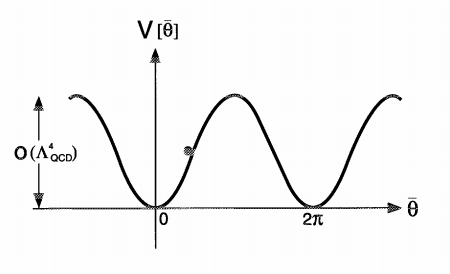
\includegraphics[width=0.6\textwidth]{vthetavstheta}
\end{figure}


\begin{figure}
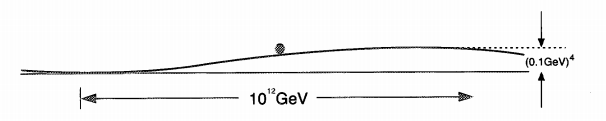
\includegraphics[width=0.6\textwidth]{axionpotential}
\caption{From \cite{kim95}; shows how slight the axion potential is.}
\end{figure}

Imagine this potential being stretched out in space, as is happening through the expansion of the universe. When the expansion slows down sufficiently so that $H \sim m_a$, the axion begins to oscillate. Because the lifetime of the axion is longer than the age of the universe, the oscillations do not die out, but the amplitude of the oscillations is decreased by the expansion of the universe. Discussion taken from Kim's "Axionic Extensions of the Standard Model".


\subsection{Models of the axion}

The first model of the axion came from introducing the new symmetry through two Higgs doublets, as proposed by Peccei and Quinn. The two doublets, $\lambda_1$ and $\lambda_2$ combine to have a non-zero vacuum expectation value. The phase of the vacuum expectation value is the axion; by current algebra techniques that mass of the axion can be computed to be 

\begin{align*}
m_a = \frac{Nm_\pi f_\pi}{v_F}\frac{\sqrt{z}}{1+z}(\frac{1}{x}+x) = (23 \text{keV})(\frac{1}{x}+x)
\end{align*}

for $ x = <\lambda_1>/<\lambda_2>$ is the ratio of the vacuum expectation values of the doublets and $z = m_u/m_d$ is the ratio of the up and down quark masses.

This Peccei-Quinn-Weinberg-Wilczek axion was predicted to have a mass of some keV, but was ruled out in reactor and accelerator experiments \cite{crystalball90} [NEEDSREF].

Simple extensions to the Peccei Quinn mechanism modified the energy scale of the symmetry breaking, decoupling it from the electroweweak scale, and allowing the axion mass to be much lighter. The Dine, Fischler, Srednicki, Zhitniskii model (DFSZ) \cite{dine81},\cite{zhitniskii81}, adds a single heavy scalar in addition to the Higgs doublets introduced before. 

The mass of the axion is then calculated to be:

\begin{align*}
m_a = \frac{f_\pi}{f_a} m_\pi N \frac{\sqrt{z}}{1+z}
\end{align*}

For $z= 0.56$, $f_\pi = 93 \text{ MeV}$, and $m_\pi = 135\text{ MeV}$, $m_a \approx \frac{10^7\text{GeV}}{f_a}eV$.

Another model, the Kim, Vainshtein, Shiman, Zakharov model \cite{kim79},\cite{shifman80}, extends the Peccei Quinn mechanism by introducing a new heavy quark and complex scalar field, as well as a discrete symmetry. The axion then couples directly to this heavy quark and through the quark, to ordinary matter. The axion mass is then:

\begin{align*}
m_a = \frac{\sqrt{z}}{1+z}m_\pi\frac{f_\pi}{f_a}
\end{align*}

and the coupling to two photons is:

\begin{align*}
g_{a\gamma\gamma}^{KSVZ} &= \frac{\alpha}{2\pi f_a}(\frac{E}{N}-\frac{2}{3}\frac{4+z}{1+z}) 
\\ &= 1.93\times10^{-15}\text{GeV}^{-1}(\frac{E}{N}-\frac{2}{3}\frac{4+z}{1+z})(\frac{m_a}{10^{-5}\text{eV}})
\end{align*}

In conclusion, for the two photon interaction for which $\mathcal{L} = g_{a\gamma\gamma}E\dot B a$, the coupling is

\begin{align*}
g_{a\gamma\gamma} &= -\frac{3\alpha}{8\pi f_a}\xi = - \frac{m_a/\text{eV}}{0.69\times10^{10}\text{ GeV}}\xi 
\\ \xi &= \frac{4}{3}(\frac{E}{N} - 1.92 \pm 0.08)
\end{align*}

$E/N$ is the ratio of the color to electromagnetic anomalies. For the DFSZ mode it is 8/3, for the KVSZ model it is 0. It cannot be guaranteed that $E/N$ does not equal 2, however, in which case the coupling to photons would be severely suppressed.


\section{Detecting axions}

Astrophysical arguments can constrain the axion mass severely. The requirement is that axions, which can produced in the cores of stars and act as an additional energy loss channel, have couplings lower than those which would produce a conflict with observation. The limits on the coupling strength to photons for globular clusters and the limit on the coupling strength to nucleons in the case of supernova SN1987A can be translated into limits on the axion mass of $m_a \leq 10^{-2} \text{eV}$ or $f_a \geq 10^9\text{GeV}$ \cite{raffelt08}.

I briefly review the techniques used to search for axions:

\begin{description}

\item \textbf{Solar axions} \hfill \\

Here one uses the Primakoff effect to search for axions produced in the sun due to the strong electric and magnetic fields in the plasma. By aiming a dipole magnet at the sun, the axions streaming from the sun can reconvert into photons (x-rays) and then be detected. The main experiment here is CAST \cite{cast11}, which has begun to edge out the globular cluster limit although not completely.  As \cite{raffelt08} notes, because the massive axions are converting to massless photons, there is a large momentum mismatch. The massive axion as momentum $k_a = (\omega^2 - m_a^2)^{1/2}$ while the photon has momentum $k_\gamma = \omega$. The difference is $q = k_\gamma - k_a \approx m_a^2/2\omega$ for $m_a \ll \omega$, so the length over which one can coherently detect a signal is limited, so conversion is a function of length.

\item{Bragg diffraction}
Another experiment used the electric fields of crystals to convert 

\item{Vacuum Birefringence}
The axion community was sparked in large part by a report of an anomalous signal in a vacuum birefringence experiment by PVLAS \cite{zavattinni06}. This experiment looked at the slight change in polarization of a laser beam in a cavity immersed a strong transverse magnetic field, which could be do to some axions being made and thus altering the polarization. When the experimenters rebuilt the experiment to reproduce the signal, however, they were unable to see the anomaly. This anomaly would have predicted an axion with mass of around 1.2 meV and two-photon coupling of 
$2.5\times10^{-6} \text{ GeV}^-1$. This patch was excluded by the BMV collaboration \cite{robilliard07}, and other photon regeneration experiments have pushed to higher laser output, and lower backgrounds to improve the sensitivity of the experiments.

\item{Rydberg Atoms}
An experiment using Rydberg atoms, CARRACK, \cite{yamamoto00}, assumed that dark matter is composed of axions. The experiment uses a strong magnetic field to convert the axions to photons in a resonant cavity. The resulting photons can excite Rydberg atoms passed through the cavity to an excited state, which can be detected using a technique called selective field ionization. They were able to get sensitivity almost to the axion model band line with a span of 8$\%$ around 10 $\mu$eV.

This technique of detection with atoms is notable because the detector is the atoms and adds no additional noise to the experiment. This will come back to haunt us when we talk about higher frequency axion detection with microwave cavities and linear amplifiers \cite{lamoreaux13}.

\item{Photon Regeneration}
Another technique looks for axions produced by the Primakoff effect from photons and a magnetic field. The axions interact weakly with matter and thus pass through an opaque barrier that will stop photons. The axions reconverting back to photons in the strong magnetic field can be detected. These experiments use strong lasers to increase their sensitivity, and do not use the assumption of axion density due to dark matter. However, the dual conversion and reconversion effects makes these processes extremely weak and difficult to detect, so the limits are well above the astrophysical bounds. Experiments with lasers \cite{ehret10}, \cite{sulc13}, \cite{chou07}, and microwaves\cite{betz13}, have placed bounds of $g < 3 \times 10^{-7} 1/$GeV for the coupling of an axion like particle to two photons.
These experiments are broadband except when using microwave cavities, and are limited only by phase mismatch which depends on the length of the interaction region. 

\item{Macroscopic Forces}
It is possible for axions to mediate spin-dependent short range forces \cite{moody84}. Experiments have been made testing this hypothesis \cite{tullney13} and finds no evidence for pseudo scalar forces as are predicted by an axion. This experiment places upper bounds on the product of two coupling factors for a certain length range; it is not straightforward to compare this to the Primakoff effect experiments, but it seems that they also have no evidence.


\item{Mossbauer Absorption}

\item{Oscillating EDMs, Dish Antennas}

\item{RF cavity}

While in the helioscopes the conversion was proportional to the length of the detector, for axions traveling along the magnetic field, for axion to photon transitions in the presence of a background magnetic field with high-Q cavities, the conversion probability depends on the overalp of the magnetic field and the electric field of the cavity mode, so thus the volume.

\end{description}

\begin{figure}
\centering
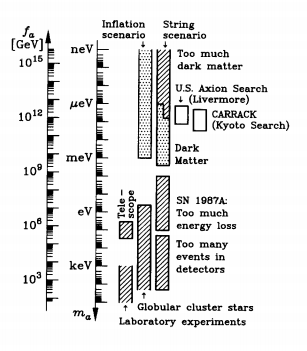
\includegraphics[width=0.6\textwidth]{1dexclusionlimit}
\caption{Constraints on the axion mass (and thus energy scale) from \cite{raffelt80}. Striped lines are constraints; blank are projected constraints; and dotted are dependent on the cosmological history of the axion.}
\end{figure}

\begin{figure}
\centering
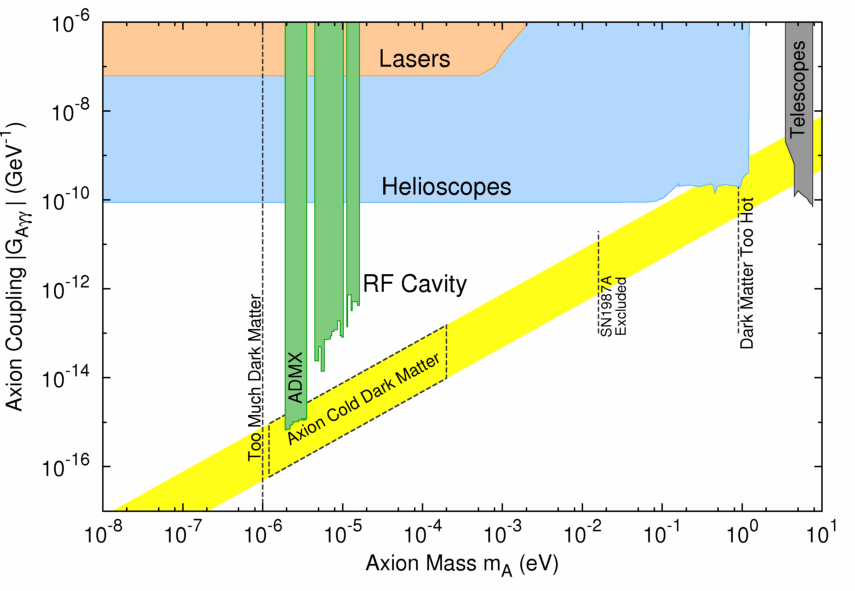
\includegraphics[width=\textwidth]{2dexclusionplot}
\caption{Summary of the ALP and axion parameter space. In yellow are shown the axion model bounds. ADMX, in green, and their experimental limits begin to constrain the axion models. Helioscopes, led by CAST, and their limits are shown in blue; photon regeneration expts labeled as Lasers exclude the upper right region but do not assume anything about dark matter so are more rigorous. The dashed line labeled SN1987A is the exclusion on the axion mass extrapolated from the observation of neutrino events from SN1987A.}
\end{figure}

\section{The Primakoff Effect}

We have referred to the Primakoff effect several times; this is the axion-two photon interaction that most axion experiments use and that is capitalized on in this work. To see how this occurs, we write the effective Lagrangian for the ALP to gluon coupling once more:

\begin{align*}
\mathcal{L} = \bar \theta g^2 G \tilde G = \frac{a}{f_a} g^2 G \tilde G
\end{align*}

This hides the fact that there is a triangle loop causing a Yukawa coupling between the axion and the intermediate fermion which couples to the gluons. Either this fermion is a heavy quark (as in the KSVZ) model, or an ordinary fermion.

The gluons can create quark-anti-quark pairs, with the pion being the lightest example. One can think of this axion-pion mixing as the effect that generates the axion mass. The pions can then decay into two photons via the Primakoff effect, which itself has a triangle loop anomaly, and this is how the axion interacts with two photons.


\section{Supernova Limit}

We make a note here about the supernova limit and how it was achieved. The limit is $6 \times 10^{-11}$ 1/GeV; better than the limits produced by this experiment. However, we appeal to systematic uncertainties in the understanding of supernova physics.

\subsection{Why microwave cavities?}
The work in this thesis describes a search for dark matter axion-like particles, using a cryogenically cooled microwave cavity in a strong magnetic field. Methods to search for these dark matter particles have been ongoing for the last four decades; however, since dark matter candidates by definition interact very feebly with ordinary matter, searching for any of these particles is experimentally challenging.  As this thesis is concerned with a dark matter axion search, I will briefly review the techniques





\section{OLD TEXT}
\subsection{Another version of Ch1}
At this point, it is firmly established that a large portion of the matter in the universe is non-luminous. Through astrophysical observations, we can estimate that the mass to light ratio in spiral galaxies is much higher than we would expect from the amount of luminous matter alone [NEEDSREF]. The existence of this gravitationally interacting matter influences the rate of structure formation in the early universe, and measurements of the cosmic microwave background can state that the observations are consistent with a $\Lambda$CDM model; that is, a model of the universe as composed of non-baryonic, non-relativistic matter [NEEDSREF]. We know very little more about this dark matter other than the conclusions stated above.

At the same time, the nature of physics at high energy (> TeV) scales is unknown. The equations that make up the Standard Model do not extend into this energy range, and current experiments that can produce physics at high energies (the LHC, other colliders) will be limited by the size of the experiments to explore energies of at most 10 TeV. Ther are many theories of physics at high energy scales; all of these predict new particles at higher energies, or additional symmetries. The high-energy particles or new effects at high energies can enter as small corrections in loop diagrams, leading to small corrections in low-energy observables. The electric dipole moment is one such observable that can be measured in laboratories but whose value is sensitive to high energy physics. The most recent measurement of the electric dipole moment of the electron \cite{acme14} done by the ACME experiment has seen a result consistent with zero, ruling out parameters of 100 TeV theories such as Supersymmetric models. These Supersymmetric (SUSY) theories are high energy theories that solve problems in high energy particle physics, and also predict a stable particle that is a very good candidate for the particle of cold dark matter.

Another probe of this high energy physics is to look for extremely light, feebly interacting particles. These particles arise as the low-mass boson accompanying the breaking of new symmetries at high energies (usually >$10^{14}$ eV). These particles, known generally as Weakly Interacting Sub-eV Particles (WISPs), are good cold dark matter candidates as well, granted that their abundance can be accounted to match the present abundance of dark matter. A particular particle belonging to the WISP category, are axion-like particles (ALPs). This denotes pseudoscalar spin 0 bosons with a non-zero coupling to two photons. ALPs take their name from the axion, a particle with the properties described above which arises from a new symmetry which was postulated by Peccei and Quinn \cite{peccei77} to solve the problem of charge and parity conservation in the theory of strong interactions when a priori there is no physical reason this CP conservation should hold.

As direct detection searches for  the SUSY dark matter candidate with no results, there is an intrinsic neutrino background that will soon limit the experiments' sensitivity within another few orders of magnitude from where they can presently search. In addition, no particles have been seen at the LHC, which expected to find new particles that would be SUSY particles. The EDM experiments have constrained different SUSY models with no observation of the electric dipole moment. At this time, it seems necessary to build small tabletop experiments that can look for other dark matter candidates, such as axion-like particles. There is a wide space in which to search for these WISPs, and having measurements allows us to constrain models. A discovery would give us clues as to the nature of physics at high energy scales, and tell us about the composition of dark matter.

\subsection{The State of Dark Matter Searches}

Starting from the assumption that dark matter is a particle, people look for heavy, stable, neutral particles, known by the acronym Weakly Interacting Massive Particles (WIMPs), under which the SUSY candidate falls. People also look for the WISPs. There are direct and indirect detection searches going on for both candidates. For WIMPS, direct searches look for WIMP to strike a nucleus, causing it to recoil. The indirect searches assume that WIMPs annihilate with each other, being their own antiparticle, and look for signatures of these events in the galaxy.

For WISPs, direct searches primarily use the ALP to two photon vertex, as it is easy to produce large electromagnetic fields in the laboratory and easy to detect photons. Searches assuming that the ALP is the dark matter are only using microwave cavities as resonant detectors \cite{admx10} although a Rydberg atom detection experiment was performed \cite{yamamoto00}. These experiments depend on the dark matter density at Earth. There are also new ideas involving the axion as inducing an oscillating electron dipole moment in nucleons \cite{budker13}, which will be sensitive to  ALPs of a different mass than those in the microwave cavity experiments. There are other experiments looking for axion-like particles, although they do not use dark matter as the source of the WISPs. These involve looking for axions produced in the sun (CAST) \cite{cast11} or directly producing axions from the two photon vertex using a laser and strong magnetic field (ALPS-I, ALPS-II) \cite{ehret10}. The direct production or light-shining-through-wall experiments has the least number of assumptions, but these experiments (solar, microwave cavity, lsw) together form a complementary way of searching for ALPs with the two-photon vertex.

There are also astrophysical arguments that can limit the coupling of the axion to the two photon vertex. The ALP, produced by various processes in red giants, neutron stars, and white dwarfs, would radiate energy from the star, altering the stellar evolution and thus stellar lifetime \cite{turner89}. By observing stellar lifetime consistent with 10$\%$, constraints on the axion coupling can be derived\cite{raffelt95}. A strong limit comes from the observation of neutrinos from the supernova explosion of SN1987A. The observation of neutrinos number and duration consistent with expectations limits the role of axions in acting as a energy loss channel. The limit is on the axion to nucelon coupling, but can be related to the axion to two photon coupling.

This dissertation will focus on a direct search for dark matter axions using microwave cavities as resonant detectors over the frequency range 33.9 to 34.5 GHz.

\subsection{Outline}

This dissertation will describe the pilot run of the Yale Microwave Cavity Experiment (YMCE) to look for dark matter ALPs in the mass range 140.2-142.7 $\mu$eV. The run set limits on the ALP-two photon coupling with sensitivity slightly better than the best previous limit set by CAST. The experiment used a microwave cavity that was tuned, immersed in a strong magnetic field - over the cavity bandwidth we would be sensitive to photons whose energy is equal to the incoming dark matter axion energy.  From the data taken, the analysis excludes axion-like particles with two-photon coupling $g_{a\gamma\gamma} < 8.6$ $1/GeV$. We end by suggesting future directions for the experiment.
The outline of the dissertation will be as follows:

\textbf{Chapter 2: Dark Matter ALPs} describes the mechanism by which these light ALPs can have the relic abundance today to match dark matter abundances observed, as well as briefly describing the specific symmetry breaking mechanism by which the axion comes about to solve the strong CP problem.

\textbf{Chapter 3: Parameter Space} goes over the current bounds on axion coupling and mass, and where microwave cavity searches fit into this field.

\textbf{Chapter 4: Detection Technique} Explains the sensitivity we can achieve using microwave cavities in strong magnetic fields, and how the expression for signal power determines what we optimize in the experiment

\textbf{Chapter 5: YMCE Experiment} goes through the components of the experiment, design of the microwave cavity, and construction of the receiver. We also go through the data taking process and summary of data taken.

\textbf{Chapter 6: Thermal Noise} The background for the experiment comes from thermal noise; we describe the expected background.

\textbf{Chapter 7: Data Analysis} puts down the analysis chain that takes the raw time domain voltage measurements and turns them into average power spectra. 

\textbf{Chapter 8: Axion Signals} We return to the expected axion power expression and walk through how that is modified when the axion energy is off resonance from the cavity resonance, but still within the cavity bandpass.

\textbf{Chapter 9:  Limits} We describe the fits and cuts applied to look for excesses in single bins that would be a hint of axion photon conversion.

\textbf{Chapter 10: Results} We present the upper bound on the ALP to two photon coupling for the mass range investigated.

\textbf{Chapter 11: Future Work} we conclude by an outlook for future work on YMCE.

\chapter{Chapter 2}
\section{Dark Matter Axion Signatures using Microwave Cavities}

The signature of a dark matter axion converting to a photon in a strong magnetic field is an excess of photons with energy equal to the axion energy. As axions are thought to be non-relativistic, this would mean that the photons would have frequency equal to the rest mass of the axion plus a small energy dispersion. The amount of this dispersion can be most simply modeled by assuming an isothermal sphere. However, if you assume cold flows of non-virialized axions, the energy dispersion becomes much smaller. The broadening of the signal peak is distorted somewhat due to earth's orbital velocity around the sun and it's own rotational velocity - these effects are at the less than 4$\%$ level \cite{rosenberg00}.

As the axion is massive and the photon is massless, there is a large momentum mismatch. By having the converted photon be an excitation of a cavity mode, this can be overcome.

The cavity also affects the rate of conversion; in a way this follows from Fermi's golden rule. In a vacuum there are isotropically many modes around; however for a cavity there are fewer modes so it is more probable for the axion to convert into the single one that is near it's energy. This is the same argument used for the Purcell effect; the phenomenon that an atom is more or less likely to spontaneously emit a photon if that transition is on resonance with a mode of the cavity.

Yet another way to think of it is as the scattering of an axion off of the cavity mode.

All in all, this makes the conversion rate go up as a factor of the cavity quality factor, Q. This property is partially what makes cavity searches so attractive. The downside though is that as we don't know the axion mass and resulting energy of the photon, we must tune the cavity resonant frequency, and are only sensitive to axions that occur with the cavity bandpass, which is inversely proportional to the Q. So with higher sensitivity to an axion at one frequency, there is less sensitivity to a wide range. This narrowband property makes for long searches. 

In this chapter, we describe the expected signal power for a photon transformed from the axion in the presence of a static magnetic field. This will depend on the cavity quality factor, the density of dark matter, and the volume of the cavity. As we will see, the cavity quality factor and volume both decrease with increasing resonance frequency, if the mode measured is the lowest mode of the cavity. Working at higher modes also brings in a cost, as the form factor which calculates the overlap of the cavity mode with the background magnetic field, decreases for higher modes.

\section{Expression for Axion Power}

o start from the theory, the axion-photon appears in the Lagrangian with an effective term as 
\begin{align*}
\mathcal{L} = \frac{1}{4}FF + \frac{1}{2}\partial_\mu a^2 -\frac{1}{2}m^2 a^2 + \frac{1}{4}gF\tilde F a
\end{align*}

where $F_{\mu\nu}$ is the electromagnetic field tensor, and $\tilde F_{\mu\nu}$ its dual; $F\tilde F = E \dot B$. This produces modified Maxwell's equations of the form \cite{hoogeveen92}:

\begin{align*}
\nabla \cdot B = 0 \
\partial_t B + \nabla \times E = 0 \
\nabla \dot E = -gB \dot \nabla a \
\partial_t E - \nabla \times B = g B \partial_t a - g E \times \nabla a \
(\partial_t^2 - \nabla^2 + m^2)a = gE\dot B \
\end{align*}

this leads to an equation of motion that, assuming a spatially uniform axion field (which in our case holds), looks like 

\begin{align*}
\nabla^2E - \partial_t^2E = gB_0\partial_t^2a
\end{align*}

where $B_0$ is the magnetic field. Decomposing the electric field in terms of the cavity modes, as well as the background magnetic field, and following the discussion in \cite{krauss85}, shows that the cavity will respond in mode j as 

\begin{align*}
\lambda_j(\omega) = \eta_j(\omega^2/(\omega^2-\omega_j^2))a(\omega)
\end{align*}

where $\eta_j$ is the fourier coefficient (with basis of cavity modes j) for describing the background magnetic field, $a(\omega)$ is the Fourier representation of $a(t)$.

Integrating over the parameter $\omega$, the energy stored in the cavity for a mode j is 

\begin{align*}
U_j = \int |{E_j(\omega,x)}|^2 d^3x d\omega \
= V \int \lambda_j^2 d\omega
\end{align*}

Including dissipation by the substitution $(\omega^2-\omega_j^2)^2 \rightarrow (\omega^2-\omega_j^2)^2 + \omega^4/Q^2$, and rewriting the $\\eta_j^2$ as $G^2B^2$ for some filling factor $G$, the energy in a mode is

\begin{align*}
U_j = G^2VB^2\int |a(\omega)|^2 \omega^4/((\omega^2-\omega_j^2)^2 + \omega^4/Q^2) d\omega
\end{align*}

On resonance, for $Q < Q_a$

$P_j = \omega_j U_j/Q = G^2B^2VQ\rho/m_a$

[ALTERNATE EXPLANATION IN TERMS OF RLC CIRCUIT]


The axion Q is, assuming virialized axions, $\sim 10^6$.

In terms of the laboratory parameters, the observable power in the $\text{�}_{020}$ mode from an axion on resonance at 34 GHz with coupling $g_{a\gamma\gamma} = 8 \times 10^{-11}$ 1/GeV would be 

\begin{multline}
P = 1.7 \times 10^{-24}\text{ W}\(\frac{C_{020}}{0.13}\)\(\frac{Q}{10^4}\) \\
\(\frac{V}{1.6\text{ cm}^3}\) \\\(\frac{B_0}{7 T}\)^2 \\
\(\frac{g_{a\gamma\gamma}}{8\times10^{-11}\text{ 1/GeV}}\)^2 \\
\(\frac{\rho_a} {0.3\text{ GeV/}\text{cm}^3}\)\(\frac{m_a}{34\text{ GHz}^{-1}}
\end{multline}

\chapter{Chapter 3}
 \section{Dark Matter ALPs}

There is strong astrophysical evidence that a large portion of the matter in our galaxy is non-luminous, meaning that it does not have electromagnetic interactions. The first evidence came from measurements by Oort \cite{oort32}, who showed that their must be more mass in the Milky Way than measured; at around the same time, Fritz Zwicky \cite{zwicky37} measured the mass to light ratio in the Coma cluster. He found that the MtoL ratio was nearly 500 times greater than that expected. Most definitively, measurements of spiral galaxies using hydrogen's hyperfine transition at 21 cm have shown that in a a survey of many glaxies, all of them have rotation curves that suggest that the matter is distributed in a diffuse halo, not concentrated near the center, as the light is\cite{rubin80}. This dark matter would affect structure formation; as pockets of local overdensity formed, non-relativistic dark matter would settle into the gravitational well and provide many sites of small structure, which could then accrete to form large structure later - this is consistent with the level of temperature anisotropies observed in the Cosmic Microwave background \cite{planck13}, and n-body simulations [NEEDSREF]. Observations of temperature anisotropies in the Cosmic Microwave Background also allow us to make predictions on cosomological parameters; $\kappa$, the geometry of the universe, and $\Omega$, the matter density. The measurement of the relative amplitude of the anisotropies tells us that the baryon density of the universe is 4$\%$. This rules out the simplest assumption that dark matter is baryonic and made of dead stars or non-luminous brown dwarfs. This was also ruled out by micro-lensing surveys of Massic Compact Halo Objects (MACHOS) [NEEDSREF], which did not find as many events as would be predicted by the abundance of dark matter. The measurements of supernova with respect to distance, using them as standard candles, tells us how much of the universe is made up on dark energy, a mysterious substance which is causing the expansion of the universe to accelerate. The amount of dark energy in the universe, taken from CMB measurements, is 73$\%$. The remaining 21$\%$ is dark matter.

The lambda cold dark matter model ($\Lambda$ CDM) supposes non-relativistic, non-baryonic particulate dark matter. 

There are three strong candidates for the particle of dark matter: sterile neutrinos, WIMPs and axions. Sterile Neutrinos are neutrinos which are right handed, and thus do not interact with the electroweak force, which only deals with left-handed neutrinos. There is some evidence for a 3.5 keV line in some galaxies which would correspond to a 7 keV sterile neutrino [NEEDSREF].

Weakly Interacting Massive Particles (WIMPs) are stable neutral particles with large mass, usually in the tens of GeV to some TeV range. These particles would have the correct dark matter density if their cross section for interactions is equal to the electroweak scale, a suggestive coincidence called the "WIMP miracle". There are also supersymmetric theories extending the Standard Model; these SUSY theories predict a super partner for every elementary particle with opposite spin, ie. every fermion has a boson partner and vice versa. SUSY theories are important for solving a problem in particle physics, which is that the Higgs mass is divergent when including higher order corrections. The lightesst SUSY partner, the neutralino, has the correct properties to be cold dark matter (spinless, chargeless) and would constitute a WIMP. There are direct and indirect searches looking for WIMPs, either through their rare scattering off of a nuclei such as LUX \cite{lux14}, or through indirect searches which assume that WIMPS are their own antiparticle and then annihilate, producing visible signatures in the galaxy [NEEDSREF]. There is some evidence from the Fermi gamma ray telescope for a WIMP like signal coming from the center of the galaxy [NEEDSREF].

Lastly, the axion is also a strongly motivated cold dark matter candidate. The axion, as described below, arises from the symmetry breaking of a symmetry introduced to solve the strong CP problem by dynamically tending the P and T violating term in QCD to zero. The axion, due to astrophysical and laboratory constraints, would need to be less than approximately 1 meV; in the models of the axion, it's coupling is related to the mass, so these light axions have extremely feeble couplings to matter, making them good dark matter candidates. They can be produced thermally, making them hot dark matter candidates, or non-thermally, either through the vacuum misalignment mechanism [NEEDSREF], through cosmic strings [NEEDSREF], or topological defects [NEEDSREF].

The argument for non-relativistic matter today usually relies on thermalization arguments; which imply that the heavier the matter, the cooler, or more non-relativistic it is today. However, there are other mechanisms by which very light particles could be produced in the early universe such that they are non-relativistic today.

\subsection{$U(1)_{PQ}$ symmetry}

To describe this mechanism we first have to describe the mechanism of symmetry breaking which gives rise to light particles. To do so, we will go through the process which gives rise to the canonical axion. This process was postulated by Peccei and Quinn in 1977 \cite{peccei77} as a natural way to produce CP conservation the theory of strong interactions, Quantum Chromodynamics. 

The Peccei-Quinn solution to this strong CP problem, as it is known, was to introduce a global chiral U(1) symmetry, denoted $U(1)_{PQ}$. This symmetry can be spontaneously broken at some energy scale $f_a$, producing massless Goldstone bosons from the azimuthal degree of freedom (this is the axion), and some high energy mode from the radial degree of freedom; this was deemed to be the two Higgs doublets in the original theory, which sets the energy scale.  There are many models that construct other scalars as the radial mode, allowing the energy scale to decouple from the electroweak scale \cite{kim79} \cite{shifman80}, \cite{dine81}, \cite{zhitnitsky80}.

The axion acquires mass through explicit symmetry breaking of the$U(1)_{PQ}$ symmetry with QCD. This occurs because of a chiral anomaly \cite{jackiw76}. In all respects this is analogous to the process by which the pion, the Goldstone boson of the axial $U(1)_A$, acquires its mass through a chiral anomaly. The mass that the axion acuqires is proportional to $m_a \sim \Lambda_{QCD}^2/f_a$. The axion coupling to matter is inversely proportional to the energy scale $f_a$ and thus proportional to the mass.

Using Higgs doublets would give one a rough prediction for the axion mass of 150 keV; this axion would have a lifetime of 1 microsecond and would have been detected in collider experiments through quarkonium decays and beam dump experiments \cite{crystalball90}. The branching ratios observed were significantly less than predicted; thus this axion was ruled out.

However, as stated above, the symmetry can come from other scalars; which would separate $f_a$ from the electroweak scale and let it be much higher, and so the axion coupling and mass would be much weaker. In 1983 Pierre Sikivie proposed using the axion to two photon coupling \cite{sikivie83} to search for axions, and proposed that axions would make good dark matter candidates. This interaction is the Primakoff effect, which can be written effectively as $E \dot B$. With strong magnetic fields, the axion to two photon transition is made much stronger.

Note, I say axion here, but these searches apply for axion-like particles in general. The only difference is that axion-like particles do not have the relationship between coupling and mass, so there are two free parameters in the theory.

In order for ALPs to be good dark matter candidates, they must have the correct abundance. We now go over how ALPs could be produced in the early universe such as to have the correct density today.

\subsection{Misalignment Mechanism}

We have covered how, by the addition of a global symmetry that has explicit symmetry breaking at some high energy scale, a low mass boson can arise. The mass of this particle will "turn on" when the energy scale at which the symmetry breaking occurs is matched in the energy scale of the universe (or more commonly described, the temperature). If we think of the initial 2$\pi$ degrees of freedom of the azimuthal mode, a simple picture would be of the tipping of the $\phi^4$ potential, or the wine bottle potential, leading to the angle to settle at one particular value. As the angle $\theta$ must approach its minimum, there will be oscillations around that point. These oscillations will be affected by the expansion of the universe; one can write a damped harmonic oscilllator equation of motion [NEEDSREF] where H is the hubble parameter.

\begin{align*}
\ddot \bar{\theta} + 3H(t)\dot \bar{\theta} + m_a^2\sin(\bar{\theta}) = 0
\end{align*}

As long as $\theta$ is not too small, these damped oscillations will result in a present day energy density roughly equal to the dark matter density we observe [NEEDSREF].

\begin{figure}
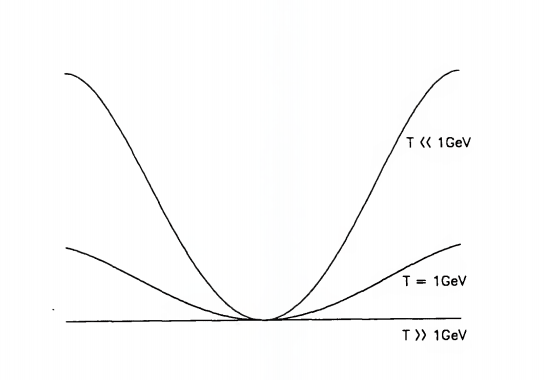
\includegraphics[width=0.7\textwidth]{differentpotentials}
\end{figure}

The cosmological history is also affected by whether the mass is turned on before or after inflation. With the 2014 BICEP result [NEEDSREF], we can set the scale of inflation at $10^{14} GeV$. If the axion acquires mass before inflation, then there is a uniform axion mass in our horizon; otherwise, there might be several causal patches with axion masses at different values, and we can only average over them to get a predicted value [NEEDSREF].


\section{Parameter Space}

When the axion mass was decoupled from its coupling, this left a 2D parameter space within which to search for the axion, from less than 100 keV in principle with no lower limit. However, astrophysical arguments have been crucial in constraining the possible parameter space for ALPs.

\subsection{Astrophysical Constraints}

The evolution of stars is limited by how fast they can get rid of the energy they create in fusion. This rate is set by the opacity of the stars; for many stars it takes $10^8$ years for photons to escape from the core to the outside. One can see that if feebly interacting particles can be produced in the star, these will freely stream out and thus radiate away more energy than just the photons could, accelerating the stellar evolution and shortening the star's lifetime.

By observing the statistical distribution of stars in globular clusters, we can infer the lifetimes of stars. They are consistent with our models of stellar lifetimes (without axions), so we can set a limit on the strength of axion coupling to matter by saying that the total energy loss (if there were axions) must be within the uncertainty of the observation. For different stars, different production mechanisms are dominant; in white dwarfs, nucleon bremmstrahlung predominates; in red giants, it is Compton-like processes [NEEDSREF].

The strongest limits come from horizontal branch stars, where Primakoff processes are strongest. These exclude axions from 1 eV and below for couplings greater than $g_{a\gamma\gamma} > 10^{-10} \text{1}/\text{GeV}$.

Another limit comes from the supernova SN1987A. Neutrinos provide the dominant source of cooling for supernovas; in less than a second, the supernova radiates all of its energy through neutrinos. If axions provide another cooling method, than we would see less neutrinos. Observations at Homestake observed nineteen neutrino events, consistent with expectations [NEEDSREF]. As the primary axion-matter interaction in supernova would be nucleon bremmstrahlung, one can exclude $g_{aNN} < 10^{-11}$ 1/GeV for axions of mass less than 2 eV [NEEDSREF]. One can convert this to a constraint on the coupling to two photons if you assume the axion obeys a particular model. The two most popular models are the DFSZ and KVSZ models, which we will now describe briefly.

\subsection{Axion Models}

After the original Peccei Quinn axion was eliminated, several models were theorized to allow for axions with different symmetry breaking energy scales other than the electroweak scale. Two are prominently refered to, the DFSZ model [NEEDSREF] and KVSZ model [NEEDSREF].

The KVSZ model introduces a new heavy quark, which couples to the axion. In this model the axion does not couple to electrons or quarks at tree-level. However it ends up having a coupling to nucleons comparable to that of the DFSZ model through other corrections.

The DFSZ model supposes that all leptons have PQ charge. This model is preferred as it fits well with GUT theories.

Both models couple to photons, through the coupling to gluons.

\subsection{Direct Searches}

Astrophysical arguments constrain a fair portion of the possible phase space; giving an upper bound on the axion mass of approximately 1 meV and an upper bound on the axion to photon coupling of $10^{-10}$ 1/GeV.

Direct searches are those which attempt to directly detect signatures of axion interactions with matter in the laboratory. Most of these searches utilize the axion to two photon coupling. One experiment, dubbed "light shining through wall" [NEEDSREF], produces axions by the combination of a strong magnetic field and laser (through the interaction term in the Lagrangian $E \dot B$. By producing an opaque barrier and then looking for excess photons on the other side which could be caused by axions traversing the barrier and reconverting into photons in the presence of the magnetic field.

Axions can also be produced by the Primakoff effect wih the strong plasmas in the sun. They can be detected by reconverting them into photons on Earth in the presence of a strong magnetic field. The CAST experiment [NEEDSREF] has done this and placed the best limits, slightly better than those of the horizontal branch star limit. The current exclusion is of $g < 8.8 \times 10^{-11}$ 1/GeV.

If axions compose the cold dark matter of our galaxy, they will have an energy density with oscillations at the frequency $m_a$ with velocity dispersion most simply described as given by the virialized velocity $v \sim 10^{-3}c$. The conversion of the axion to photon in the presence of the magnetic field will then deposit all of the axion energy into the photon, creating photons with frequency $\nu \sim m_a$. By having the conversion take place in a resonant cavity with a mode resonant at $m_a$, the signal will coherently build up by a factor of the cavity quality factor Q. This technique of resonant detection, assuming a strong source of axions from dark matter, can achieve high sensitivities. This is the technique used in this thesis. The main work done in this has been by the ADMX experiment [NEEDSREF] which has excluded KVSZ axions for mass of 1.9 to 3.5 microeV. Future work is ongoing by them to cover more frequencies, possibly up to 80 $\mu$eV.

Other methods using Rydberg atoms, and methods not utilizing the Primakoff effect have been proposed or performed [NEEDSREF].

\chapter{Chapter 4}
\section{Detection Technique}

Despite having referred to the Primakoff effect and cavity detection of dark matter axions previously, we know set down the expressions governing the expected sensitivity and show the effective Lagrangian.

\subsection{Lagrangian}

To start from the theory, the axion appears in the Lagrangian as 
\begin{eqnarray}
[NEEDSEQN]
\end{eqnarray}

where $F_{\mu\nu}$ is the electromagnetic field tensor, and $\tilde F_{\mu\nu}$ its dual. This produces modified Maxwell's equations of the form

\begin{eqnarray}
[NEEDSEQN]
\end{eqnarray}

The effect on the microwave cavity on the signal power can be derived by decomposing the fields in the cavity as modes and plugging them back into the modified wave equation [NEEDSREF]

A physical way to see this is to rewrite the microwave cavity as an LC resonator being driven with a voltage oscillating at $m_a$ (the axion).

We assume a Maxwell-Boltzmann distribution of the axion energies, boosted by the velocity of the earth [NEEDSREF].

The form factor expresses the amount of overlap between the electric field in the cavity mode and the dark matter axion field, with the following equation:

\begin{eqnarray}
[NEEDSEQN]
\end{eqnarray}

The form factor is zero except for modes of the form $TM_{0n0}$, and goes as 1/$n^2$, so sticking to modes with low index is favorable.

The two approaches yield the same result: the energy in the cavity on resonance as a result of the axion photon conversion is:

\begin{eqnarray}
[NEEDSEQN]
\end{eqnarray}

The power is given by $P = U\omega/Q$ and so the power expected is

\begin{eqnarray}
[NEEDSEQN]
\end{eqnarray}

Re-written in terms of the laboratory parameters, this gives us an expected signal power of $10^{-17}$ W coming out of the cavity for the following experimental values:

\begin{eqnarray}
[NEEDSEQN]
\end{eqnarray}

From the sensitivity expression one can see that maximizing the magnetic field will yield the greatest improvement. The value of the quality factor can be analytically calculated; it is a function of the skin depth and frequency, and goes as:

\begin{eqnarray}
[NEEDSEQN]
\end{eqnarray}

In our experiment we operate at frequencies of 34 GHz. Our empirical loaded quality factors are close to the analytical prediction.

\chapter{Chapter 5}
\section{The Magnet and Cryogenic Systems}




%The tuning rod connection consists of a bellows which allows the rod to enter a vacuum compatible region that has vertical motion capability.


%
%The cryostat is a gas flow design, meaning the primary mechanism of cooling occurs through convection? Movement of the helium gas from the bottom where it is boiling off from the liquid collected to the top. The atmospheric valve is left open so that when running the cryostat has slightly more than atmospheric pressure. There are several circular mylar baffles in place as well.


The experiment consists of a microwave cavity in the bore of a superconducting solenoid magnet from Oxford Instruments. The magnet is made of  NbTi alloy with copper windings and has a maximum field of 7 Tesla. The warm bore has a diameter of 89 mm. Over the size of the cavity the magnetic field is homogenous to better than $1\%$.

\begin{figure}[htbp]
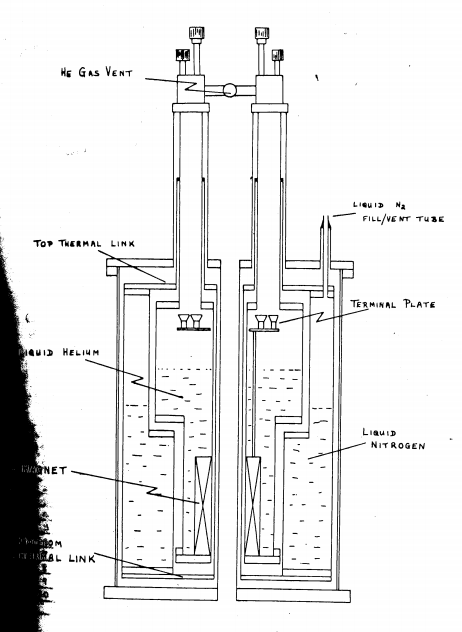
\includegraphics[width=\textwidth]{nmrmagnet}
\caption{Oxford instruments NMR magnet}
\end{figure}

The magnet was cooled in the summer of 2011 and has run in persistent mode at full field up to the time of writing. A separate gas-flow cryostat custom built from Cryo Industries sits in the bore. This cryostat has an inner diameter of 1.57 inches and is offset from the bore center so that there is enough space for a second cavity to sit in the bore, outside the cryostat. 

\begin{figure}[htbp]
\centering
\includegraphics[width=1.3\textwidth, angle = 90]{cryostatalltogether}
\caption{Top half of the cryostat, with inset showing full cryostat. The cavity is located at the bottom of the sample region above the vaporizer}
\end{figure}

There are 3 Liter reservoirs for nitrogen and helium at the top, and a touch point with the nitrogen reservoir halfway down. A capillary tube allows liquid helium to flow from the reservoir to the bottom of the cryostat, and a block with a heating element inside of it allows us to control the temperature of the cryostat. We found when running that the temperature stability of the system as well as the helium consumption depended heavily on the cryostat vacuum - if we ran for more than two weeks, the helium consumption would more than double, from 30 L/week to 70 L/week. Thus during the actual runs we had to pump out the cryostat vacuum insulation layer every other weekend. 

A typical cooldown consists of filling the nitrogen reservoir of the cryostat, which we can do automatically through an autofill mechanism, clearing the capillary line from any air or nitrogen by running helium gas through from the helium reservoir, opening the flow valve and pumping on it, and then filling the helium reservoir. To go from room temperature to 4 K at the bottom of the dewar generally takes about three hours. If we do this procedure the night before, when we fill the nitrogen and helium again the next day it only takes an hour, generally.

%There are two cryogenic amplifiers with a gain of 50 dB and waveguides WR28 carry the signal power out of the cryostat to a room temperature electronics chain which filters, amplifies, and mixes the signal down to baseband, so it can be digitized. We have a PCI- National Instruments (PCI-5114) digitizer that samples at a rate of 10 MHz second, with a 10 MHz digital signal sent in by the PXA Signal Analyzer N90330A which is in turn phase locked to the first signal generator, which outputs a 10 MHz analog signal. A test tone signal is generated by a second signal generator, also an Anritsu MG3694C, offset to 3 MHz lower than the cavity resonant frequency. There is an RF switch (model number) to connect either one cable of the network analyzer (also frequency locked) or to take the signal power to the receiver. There is another RF switch on the other cable of the network analyzer that connects either the test tone signal to the calibration port or the network analyzer input. 

\begin{figure}[htbp]
\includegraphics[width=\textwidth]{closeupschematic2}
\caption{Not to scale. Sketch of cavity and waveguides in cryostat. Helium enters the sample region at the vaporizer; a heating element can be adjusted to increase the boil-off rate and thus raise or cool the cryostat temperature.}
\end{figure}

The heat load into the dewar is dominated by the waveguides. The two WR28 waveguides in the insert have Mylar radiation baffles to reduce any radiation heat load coming from the top, and a six inch section of copper-clad stainless steel WR28 at the top to also help reduce the heat load. There are two flexible 3 inch sections of WR28 waveguide that allow us to connect to bulkheads feedthroughs. An electrical stock allows electrical wires to go through for temperature sensors. 
The tuning rod consists of a G-10 rod, .125" diameter. The waveguides are made of several pieces - at the top of the insert there is a six inch section of stainless steel copper coated waveguide, and the rest is copper waveguide. This is to reduce the heat load on the bottom of the cryostat. The waveguides used throughout are WR28 - which means rectangular waveguide with a lower cutoff frequency of 21.5 GHz.
We place the assembly of the cavity, low noise cryogenic amplifier, and waveguides, which we call the insert, into the cryostat with a vacuum seal at the top. There are several temperature sensors and the power leads for the LNA is also fed through.
I should also mention that the tuning mechanism, which in this case consists of a long rod that is attached at the top via a screw, is coupled in a vacuum compatible way. The waveguide and cavity together consist a closed system - we pump on the waveguides when trying to keep liquid helium from entering the cavity, which it can do most probably through the tuning rod connection. 



%Another danger is if the cavity gets liquid in it, the resonance is no longer stable. This is probably because it fills up very slowly due to a small but intermittent leak somewhere in the indium seals of the waveguides. This means that whenever we saw the temperature sensors reading less than 4 K, we usually stopped the run and heated the cavity up. Thirdly, we found that the stability of the cavity resonance was more robust to changes if the cavity was at a higher temperature - changes of .5 K at 10 K seemed to affect the cavity resonance much less than at 5 K. One explanation is that the pressure in the cavity altered the resonance frequency - from John Rogers Thesis \cite{rogers87}, in their experiment they saw that there was a 30 kHz/GHz/psi shift. We see a XXX shift.




\section{The Microwave Cavity}

\subsection{Design}

We use a cylindrical cavity built out of oxygen free high conductivity (OFHC) copper, which consists of a block with a machined cylinder and a bottom end cap. After machining, the surfaces were polished with a rouge polish to reduce the roughness.  The pieces were then screwed together with an indium seal in between, and a taper cut into the bottom cap in order to allow for the spreading out of the indium as it compressed. 

%This will go into a previous chapter \subsection{Why � 020}
%The reason we have been talking about TM020 all this time is because the Tm010 mode has too small a size in the 34 GHz range. Let us expand our range and take the entire Ka-band, or R-band as it is sometimes called. From 26.5-40 GHz, if the Tm010's resonant frequency lies in that range, it's cavity radius would be 4.33 mm to 2.869 mm. Hmm that actually seems pretty ok for the lower range. Why are we workign at 34 GHz anyways? The Tm020 mode would have 9.9mm-6.58mm. The size of our current opening in the cryostat is 40 mm. Our current cavity has a radius of 5 mm in the Te011 mode.
%However! We believe that the TM020 mode has a higher Q, at least theoretically, which with the higher volume for the same frequency, actually compensates the degraded C (C for 010 is 0.69 and C for 020 is 0.13). Although there are more mode crossings, we don't worry about this because we make the cavity height sufficiently small so that other modes can't come in.
%The reason we are working above 20 GHz is because this region is as of yet unexplored. People have been using large microwave cavities to look for lower mass axions because of the higher sensitivity due to the large volume. It is our goal to push the exploration to higher masses in order to investigate possible axion-photon couplings in this as of yet unexplored region.
%The reason we are working precisely at 34 GHz is pretty stupid though. We wanted to use a high power pulsed source which puts out fixed frequency 34.29 GHz radiation. Then we designed our whole system around it and now don't want to change it because it would be a pain.
%Our other limitations are the present waveguides installed (fundamental mode operates between 21.5 and 40 GHz even though the rating says 26.5-40 GHz) and the RF filter. Also our electronics might not be happy. But the LNAs can go from 11-34 GHz.
%We mention here that we are tryng to do something that cavities are not really made to do - be a broadband detector. They are very good at picking out specific frequencies from a broadband input, or enhancing processes when the radiation these processes emit is at a frequency where the cavity resonates. So much work is being done trying to bring tuning, which is a slow process with a cavity, into the picture.

\subsection{Aperture Coupling}
There are two coupling holes - the first one is to couple power out of the cavity. For critical coupling, the power coupled out is equal to the power lost in the walls. This gives optimal signal to noise. The other hole is so that we can send in power in order to do transmission measurements, which allow us to determine the Q of the cavity and the resonant frequency. This hole is in general very weakly coupled $<50 dB$. 

%We use coupling holes instead of antennas for god knows why. The reason is at the frequency we work at it is problematic using cables. They are lossier than waveguide and I don't know what else.

We couple inductively by picking up overlap in the magnetic field of the waveguide mode (TE(10) and the azimuthal field of the cavity TM020 mode. As discussed in the previous chapter, operating in the TM020 mode decreases the form factor C from the maximal value, but allows us to have a larger volume, which increases the sensitivity. It is also easier to machine and work with a cavity that is larger than the waveguides. The TM0n0 modes have only non-zero electric field in the z direction 

\begin{align}
E = E_0 J_0(x_{0n} r/R) e^{-i\omega t} \hat{z}\\
B = -i\sqrt{\epsilon}E_0J_n(x_{0n} r/R) e^{-i\omega t}\hat{\phi}
\end{align}

where $x_{0n}$ is 0th root of the nth Bessel function $J_n$ and R is the cavity radius.  The cavity resonant frequency is 

\begin{align}
\omega = \frac{5.52}{\sqrt{\epsilon}} \frac{c}{R}
\end{align}

where $x_{02} = 5.52$.

%There is no intrinsic advantage to this, just that the geometry of the fields in the waveguide and in the cavity and our space constraints make it easier to have vertical waveguides on the sides of the cavity and the fields in the mode that align with the propagating fundamental mode of the waveguide happen to be magnetic ones.

The TM020 mode must have good connection between the walls and the caps because the alternating E field means that there are vertical currents that switch direction and flow in the vertical axis so if they cannot flow to the top or bottom cap, the mode's Q will be severely degraded.
%\subsubsection{HFSS}
%Shown below is a cross-sectional plot of the electric field in the z-direction for a dielectric rod with $\epsilon = 9.2$ inserted 0.028 inches into the cavity.
%
%\begin{figure}[htbp]
%\centering
%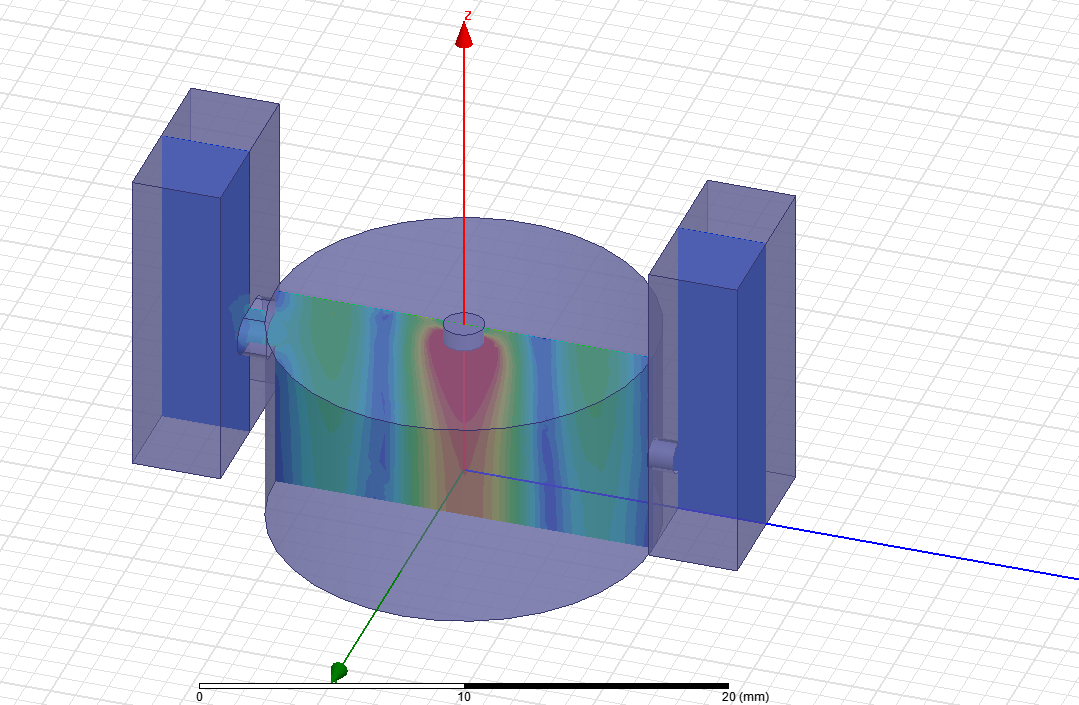
\includegraphics[width=\textwidth]{efieldhfsssim28thou}
%\caption{Magnitude of Electric field in the mode with dielectric rod inserted.}
%\end{figure}

\begin{figure}[htbp]
\centering
\includegraphics[width=0.6\textwidth]{tm020efield}
\caption{Electric field lines in the cavity.}
\end{figure}

\begin{figure}[htbp]
\centering
\includegraphics[width=0.6\textwidth]{tm020magneticfield}
\caption{Magnetic field lines in the cavity.}
\end{figure}

\begin{figure}[htbp]
\centering
\includegraphics[width=\textwidth]{waveguidefields}
\caption{Showing the magnetic field lines of the $TE_{01}$ propagating mode in the waveguide. This couples to the azimuthal magnetic fields in the cavity.}
\end{figure}
\subsection{Tuning}
%The cavities we use for detection are made to resonate at frequencies near $~34$ GHz. This choice has to do with the predictions for the resonant frequency of axions, sensitivity, and the constraints on making 3D cavities that will fit into the space limitations of our current setup.

Taking the most practical consideration, the diameter of cavities scale in size as $\lambda$. We assume throughout we are only interested in low order modes for which the prefactor for lambda is O(1). If we wish to tune the resonant frequency of a particular mode, the common methods are perturbing the cavity geometry, either by inserting a dielectric or physically changing the size of the cavity. 

For axion searches, only $\text{TM}_{0n0}$ modes couple to the emitted photon, and the frequency is independent of the cavity height, which is easier to adjust than the radial dimension. 

%Therefore the scheme that we use for our $TE_{011}$ cavity of using a floating cap that we can vary the height of (called the plunger) no longer works.  

So instead we introduce a dielectric, in our case alumina ceramic which has a relative permittivity of $\epsilon \approx 9.3$. The size of the dielectric will affect how much it perturbs the cavity mode - in our case we limited the size of the dielectric rod by considering what the cutoff frequency was of the tube in which the dielectric was held. For a circular tube (which is essentially a waveguide) with $\epsilon = 9.3$, light will not propagate until 36.22 GHz for a diameter of 0.063". 

In order to keep the mode Q high, it is best not to destroy the axial symmetry of the $TM_{0n0}$ mode so we insert it vertically in the center. It is also easier to make vertical insertions that horizontal ones, where the cavity must be aligned with its axis along the axis of the magnet. 

Not only the resonance frequency, but the form factor C will be affected by the dielectric since the fields in the mode are perturbed. Other groups (ADMX) have seen that inserting a dielectric rod can cause large degradation in the field mode, however we do not find this to be the case in our simulations for the range of insertion depths tested. 

\begin{figure}[htbp]
\centering
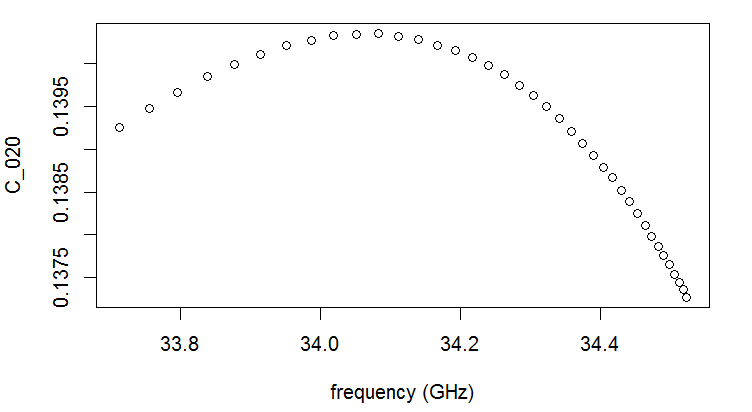
\includegraphics[width=1\textwidth]{formfactorvsfrequency}
\caption{Form factor calculated for an axially moving dielectric rod of radius .0315 in and cavity radius $R=.3$ in. The frequency span is reached for a travel of 0.032 in of the dielectric rod.}
\end{figure}

The height of the cavity was set to be $L=0.34$ in to avoid a mode crossing with the higher TE112 mode that appeared in the simulation. However, when the cavity was built the modes were separated by at least 2 GHz and there is no danger of a mode crossing over the range in which we scan. The other close mode is the TM010 mode, which is at 17 GHz.

\begin{table}[htbp]
\caption{Summary of cavity parameters}
\begin{center}
\begin{tabular}{|c|c|c|c|c}
\hline
R [in] & tuning rod & tuning range [GHz] & $Q_{wall}$ & C \\ \hline
0.3 & dielectric & 33.9-34.5 & $1.9\times10^4$ & 0.13 \\ \hline
\end{tabular}
\end{center}
\label{summary}
\end{table}%


\subsection{Simulation and Bench Tests}
\subsubsection{RF Properties at Cryogenic Temperatures}
%The walls of the cavity are 40 thousandths thick at their thinnest point. There is a small hole for the weak coupling port and a large oval ``racetrack`` hole for the strong port.  

The cavity was simulated in Ansoft HFSS. Surface finish plays a large role in the Q of the cavity - using a surface roughness tester we determined that the surface roughness of the cavity surface was less than 2 $\mu$inches. This value leads to negligible effects in the simulations and was therefore neglected.  

$\sigma = 5.86 \times 10^{7}/\Omega\cdot\text{cm}$ for oxygen-free copper at 294 K.

At cryogenic temperatures the conductivity of copper is approximately three times higher. The regime of low temperatures and microwave frequencies causes the anomalous skin depth effect - where due to the fact that the mean free path is now longer than the skin depth, one can no longer use the classical formula for the conductivity. In this regime the skin depth is given by:

\begin{align}
\delta = \big(\frac{\sqrt{3}c^2 m_e v_F}{8\pi^2 \omega n e^2}\big)^{1/3}
\end{align}

where $m_e$ is the electron mass, $e$ the electron charge, $v_F$ the Fermi velocity, and n the conduction density \cite{hagmann90}. For copper, $v_F  = 1.57 \times 10^8$ cm/sec and $n = 8.5 \times 10^22\text{ cm}^{-3}$, so the anomalous skin depth is 

\begin{align}
\delta = 2.8 \times 10^{-5}\text{ cm} (\frac{GHz}{f})^{1/3}
\end{align}

For the $TM_{010}$ modes the theoretical unloaded Q is $$Q_0 = \frac{L}{L+R}\frac{R}{\delta}$$

in general a cylindrical $TM_{mnp}$ mode has Q equal to \cite{poole96}

\begin{align}
Q_0 = \frac{\lambda}{\delta}\frac{[x_{mn}^2 + (p\pi a/d)^2]^{1/2}}{2\pi(1+2a/d)}
\end{align}

 where a is the radius and d the length. Then for the $TM_{020}$ mode, this simplifies to 
 \begin{align}
 Q_0 =\frac{\lambda}{\delta}\frac{5.52}{2\pi(1+2a/d)}
 \end{align}
 
 and recall that at room temperature, the skin depth is given by 
 
 \begin{align}
 \delta= (2/\omega \mu \sigma)^{1/2}
 \end{align}

The theoretical unloaded Q in the anomalous skin depth regime for the $\text{�}_{020}$ mode with $2a/d = 1.76$ and $\lambda = .88\text{ cm}$ ($f=34$ GHz) is:

\begin{align}
Q_0 =\frac{.88\text{ cm}}{8.6\times10^{-6} \text{ cm}}\frac{5.52}{2\pi(1+1.76)} = 3.2\times10^4
\end{align}
 
 and at room temperature assuming resistivity of 1.69 $\mu\Omega \text{ cm}$,
 
 \begin{align}
 Q_0 =\frac{.88\text{ cm}}{11.2\times10^{-6} \text{ cm}}\frac{5.52}{2\pi(1+1.76)} = 2.5\times10^4
 \end{align}
 
 We measure the unloaded Q to be $1.9\times10^4$ and $1\times10^4$, respectively for the cold and warm cases. The loaded Q goes from 6455 to 9422, and the coupling coefficient goes from 0.6 (warm) to 1.15 (77K). Measurements of the coupling coefficient as the cavity is tuned (warm) show that it varies by 15$\%$ over the frequency range.  We take 1.15 to be the coupling coefficient at liquid helium temperatures. The VNA estimates the loaded Q here by finding the 3 dB bandwidth about the cavity peak in the transmission measurement. This is slightly inaccurate as the cavity is not critically coupled, but as an approximation is satisfactory for our purposes and we take the Q measured this way as the loaded Q during data runs.
 
%  In general $Q_0(TM_{0n0}) \sim x_{0n} \lambda/\delta $ for the aspect ratio kept constant.
% As $x_{mn} \sim n$ and $\lambda/\delta \propto f^{-3/2}$ or $f^{-4/3}$ depending on the regime, if you had to decide on what mode to operate in at a particular frequency, taking into account the axion signal power at $m_a=f$ being proportional to $C_{0n0}VQ/m_a \propto n^{-1} (n/f)^{3} Q/f \propto n^{3}$ implies going to higher order modes is more advantageous for operating at a fixed frequency. However the density of modes also increases proportionally to $n$, so the number of mode crossings will make the experiment difficult.

%Two cavities were made - the difference between them being that the small hole was .052 or .05, and that the length between the center of the hole and the ledge on which the waveguides rested was .06 or .08 inches. Both of these parameters should have given equivalent cavities, but when tested, it was seen that the first cavity had a worse Q (it had a rougher finish) but was also much more overcoupled. However, the loss through the weak port was -50 dB as expected. The second cavity had a higher Q, was less overcoupled (although still slightly overcoupled), but had a much higher loss of -68 dB. 

\begin{figure}[htbp]
\begin{subfigure}{\textwidth}
\centering
\includegraphics[width=\textwidth]{warms11}
\caption{Room temp�rature cavity frequency, Q, and coupling. Plot of reflection coefficient $|\Gamma|^2$ vs detuning from resonance $f_{\text{res}}$. Unloaded Q and coupling coefficient calculated via formula in Ref \cite{kajfez94}}
\end{subfigure}
\begin{subfigure}{\textwidth}
\centering
\includegraphics[width=\textwidth]{colds11}
\caption{Cavity at 77 K in liquid nitrogen.}
\end{subfigure}
\end{figure}

 The cavity was designed so that there would be no mode crossings within the frequencies scanned.  The resonance frequency shifts by 100 MHz from 34.407 to 34.517 GHz (dielectric rod not full retracted) when going from room temperature to 77 K; this is consistent with the thermal contraction of copper, whose fractional expansion coefficient in going from room temperature to 4 K is $\Delta L/L = 0.324\%$ Ref \ref{jackekin}.
 
 \begin{figure}[htbp]
\includegraphics[width=\textwidth]{1}
\caption{Cavity trace from VNA at room temperature.}
\end{figure}
\begin{figure}
\includegraphics[width=\textwidth]{20}
\caption{Cavity trace from VNA when cooled to 77 K.}
\end{figure}


 \begin{figure}
 \begin{subfigure}{\linewidth}
\includegraphics[width=\linewidth]{chart_5(3)}
\caption{Tuning (warm): loaded Q vs frequency}
\end{subfigure}
\begin{subfigure}{\linewidth}
\includegraphics[width=\linewidth]{chart_8}
\caption{Tuning (warm): frequency vs rod insertion depth}
\end{subfigure}
\end{figure}

%\begin{figure}[htbp]
%\includegraphics[width=\linewidth]{chart_7}
%\caption{Bench tests (warm): coupling coefficient vs frequency}
%\end{figure}

%Although it is impossible to perform the same test with the cavity in situ because we cannot make a reflection measurement on the strong port (we don't have space to put in a directional coupler), we see that the loaded Q is THIS at 4 K. 

%PLOT OF SIMULATED FREQ COLD AND ACTUAL FREQ COLD

%The simulation predicts that going from warm to cold, the thermal contraction taken into account and keeping the conductivity the same, that you should get so much change in the coupling and frequency.

%The simulation predicts that you can tune over a XXX frequency range without a mode crossing. It also predicts that the Q should degrade by YYY over a certain range. The form factor is predicted to be ZZZ. What we see in practice is that there is a mode crossing (warm); in situ, there is a blind spot. The upper and lower modes should be TE112 and TM010.

\subsection{Assembly with Tuning Mechanism}
The cavity is a right circular cylinder made of OFHC copper. The cavity has two aperture couplings on the side - these apertures go to WR28 waveguide, which is soldered on. The cavity has a removable bottom lid, which can be screwed on with 2-56 screws with Belleville washers - it has a groove for an indium seal, with the outer lip of the groove tapered off. This ensures the contact happens between the inner lip of the groove and the cavity bottom.

The cavity assembly consists of the cavity body, two waveguides, and tuning sub-assembly. The tuning rod is an alumina dielectric rod with dielectric $\epsilon = 9.2$. The loss tangent from the literature is $< 10^{-5}$ at Ka-band frequencies and thus can be neglected in comparison to the loss due to the walls: $1/Q_0 \approx 10^{-4}$.

The tuning rod is held in place with a pin socket which is press fit to a copper disk. A BeCu bellows is brazed to this disk, and the bellows itself is encased in a sleeve. The rod is moved by force from above; a lever arm translates the off-center motion of a G-10 rod rotating on a 100 threads per inch fitting into vertical motion on the rod. The range of the lever arm is 16.9$\deg$ for a total of .185 inches of rod travel.

At room temperature the assembly was tested for vacuum leaks. Weak points were the solder joints between the waveguides and the cavity body, the brazing joints holding the bellows to the outer caps. These joints were resoldered or re-brazed until the assembly had no vacuum leaks at room temperature.

\begin{figure}[htbp]
\centering
\includegraphics[width=\textwidth]{full-thing}
\caption{Cavity Assembly}
\end{figure}

\begin{figure}[htbp]

%\begin{subfigure}{0.5\textwidth}
%\includegraphics[width=\textwidth]{bellows-subassembly}
%\caption{Bellows sub-assembly showing bellows cap and o-ring}
%\end{subfigure}
%\begin{subfigure}{0.5\textwidth}
%\includegraphics[width=\textwidth]{top-view}
%\caption{Top-view}
%\end{subfigure}
\begin{subfigure}{\textwidth}
\centering
\includegraphics[width=\textwidth]{bellows-subassembly2}
\caption{Bellows-sub-assembly}
\end{subfigure}
\begin{subfigure}{\textwidth}
\centering
\includegraphics[width=\textwidth]{outline}
\caption{Cavity body and Waveguides}
\end{subfigure}
\begin{subfigure}{\textwidth}
\centering
\includegraphics[width=0.58\textwidth, angle = -90]{cavity-outline}
\caption{Cavity body}
\end{subfigure}
\end{figure}

%\begin{figure}[htbp]
%\includegraphics[width=0.76\textwidth,angle=-90]{cavitylaidout}
%\end{figure}

%\begin{figure}[htbp]
%\begin{subfigure}{0.4\textwidth}
%\includegraphics[width=\textwidth]{hemts}
%\caption{Waveguide to coax adaptor and two HEMTs with 3 dB attenuation between them. The adaptors have been potted with forr seal to make them vacuum tight.}
%\end{subfigure}
%\begin{subfigure}{0.4\textwidth}
%\end{subfigure}
%\begin{subfigure}{0.3\textwidth}
%\includegraphics[width=\textwidth]{bottomofinsert}
%\caption{Insert shown without amplifiers. Cavity is connected to tuning mechanism and waveguides.}
%\end{subfigure}
%\end{figure}

%\begin{figure}[htbp]
%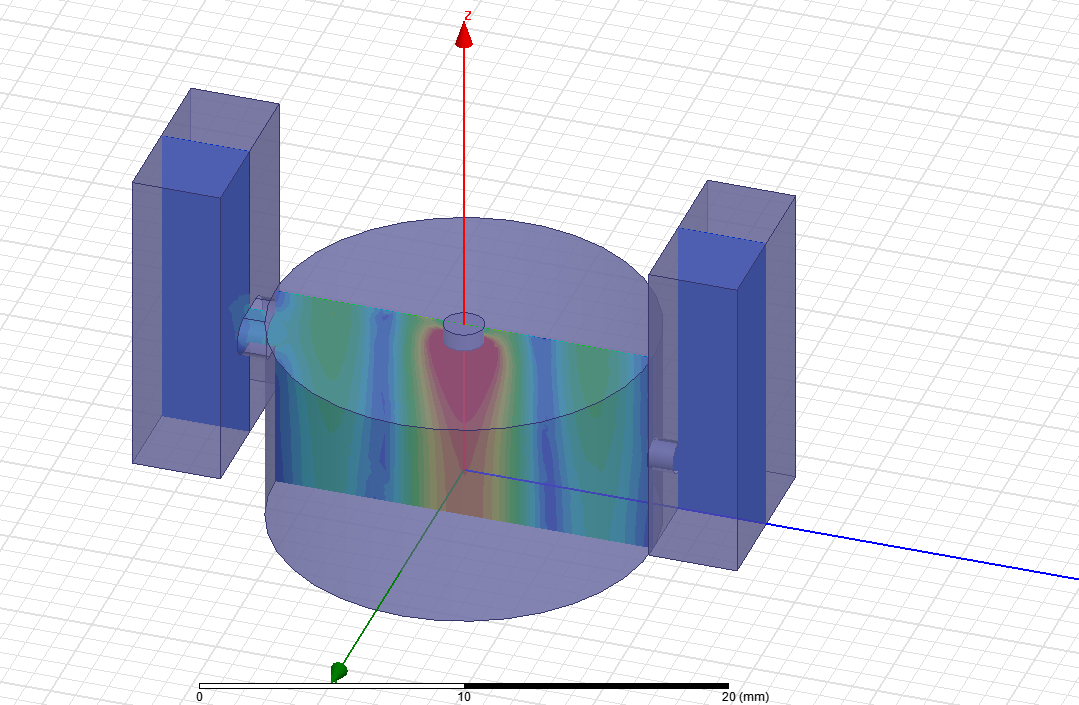
\includegraphics[width=0.6\textwidth]{efieldhfsssim28thou}
%\caption{HFSS Simulation of electric field magnitude in the $TM_{020}$ mode of the cavity.}
%\end{figure}


%The theoretical unloaded Q \ref{rogers89}:
%
%$$Q_0 = \frac{\mu}{\mu_c} (\frac{\mu_c \omega \sigma}{2})^{1/2} \frac{V}{S} \cdot 2 $$
%
%$\mu$ and $\mu_c$ are the permeabilities of the cavity interior and walls in MKS units, which are nearly equal to $\mu_0$ for helium and copper: $\omega$ is the resonant frequency and $\sigma$ the conductivity of the walls.

%\begin{figure}[htbp]
%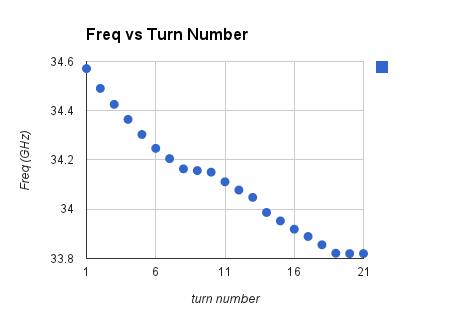
\includegraphics[scale=0.7]{freq_vs_turn_number}
%\caption{TE mode freq tuning}
%\end{figure}

We tune using a 1/16th inch thick dielectric rod ordered from McMaster, with the suppliers originally being Coorstek. THis alumina rod is secured with a pin socket soldered to a copper top hat. This has a groove for an indium seal and this hat is screwed on to the top face of the cavity. There is a small beryllium copper bellows soldered on to the top of the top hat, and this is encased in a tube which provides structural support to make sure the bellows only has one degree of freedom in the vertical direction. 

There is a lever arm that pushes the bellows up or down - this is controlled by a G-10 tube that connects from a screw at the top of the cryostat which we manually turn, and thus allows us to translate the rotation motion into translational motion of the lever arm. 

%\begin{figure}[htbp]
%\centering
%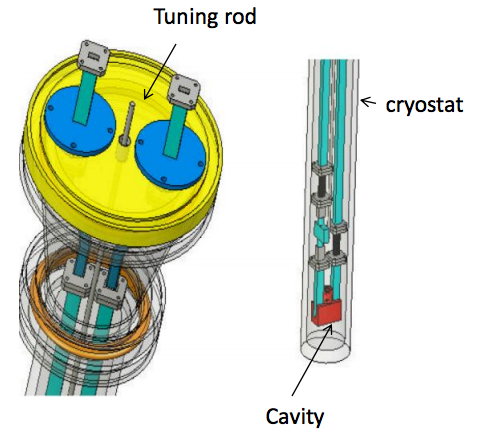
\includegraphics[width=0.7\textwidth]{insertdrawing}
%\caption{Model of the insert, showing cavity at bottom}
%\end{figure}
%\begin{figure}[htbp]
%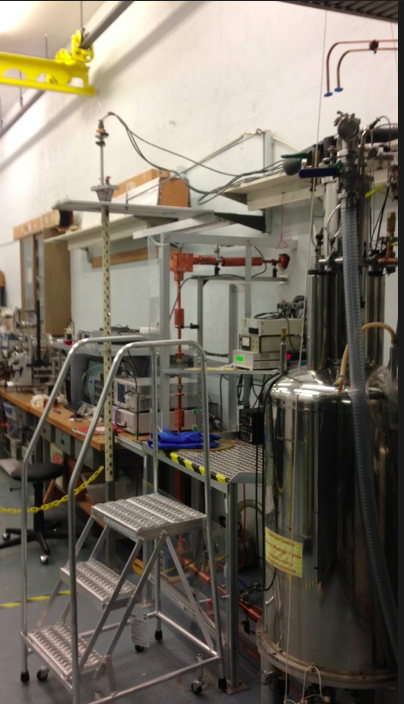
\includegraphics[width=0.8\textwidth]{experiment}
%\caption{Picture of cryostat bolted onto magnet, with insert in background.}
%\end{figure}


\section{The HEMTs}

The low noise amplifiers are placed in the cryostat and are High Electron Mobility Transistors (HEMTs). We have two cascaded together, with a three dB attenuator between them. The first amplifier (both were ordered from Sandy Weinreb at Caltech) was measured by him to have a minimal noise temperature of 35 K at a physical temperature of 15 K and 34.3 GHz, and a noise temperature of 150  K at room temperature. The second amplifier has slightly worse characteristics - the noise temperature at 15 K is given as 90 K and at room temperatue it is 168 K (we only have room temperature data up to 26 GHz). The gain for the optimal voltage settings to operate cryogenically are given by Sandy Weinreb as $32.2 \pm .2$ dB for the first and $27.5 \pm .2$ dB for the second.

\begin{figure}[htbp]
\includegraphics[width=\textwidth]{weinrebgain}
\caption{Gain of 1st amplifier measured by vendor}
\end{figure}

Put in the VNA screenshot of the amplifier gain at room temperature here.

There are two HEMT voltage settings that produce an optimal gain/noise combination for the different temperatures. We adjust the voltage (adjusting for resistive losses due to the cables between the power supplies) for the cold setting during cool-downs.

 
We measured the noise temperature of the first cryogenic amplifier by doing a Y-factor measurement. This meant using a $50$ ohm RF termination as noise source and varying the temperature while keeping the HEMT thermally isolated. We did this by connecting the termination to the HEMT via a two and a half inch long piece of stainless steel co-axial cable. The termination was encased in a copper block, which had a central hole through which a carbon resistor of 1 k$\Omega$ was placed, with thermal grease applied to increase the contact between the copper block and resistor. Current was injected into the resistor which heated the copper block and thus the terminator; by measuring the difference in the output noise power we can extract the amplifier intrinsic noise temperature. The electrical loss of the stainless steel coax segment was measured to be 0.5 dB and included in the calculations.

\begin{figure}[htbp]
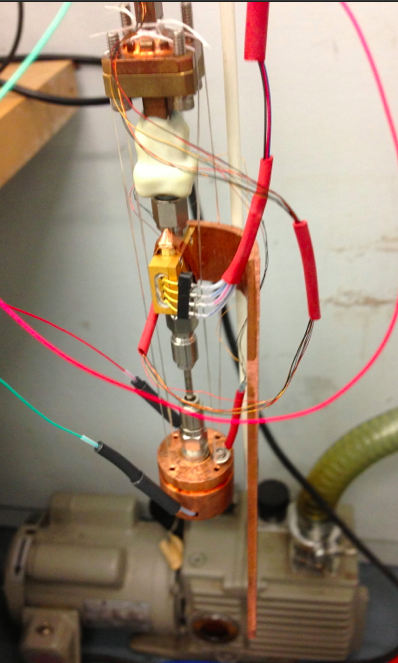
\includegraphics[width=0.6\textwidth]{noisetempmeasurement}
\caption{Photograph showing copper block and first amplifier. The heating element is a 100 k$\Omega$ resistor threaded through the block. A cold finger is attached to the amplifier.}
\end{figure}

$P_{out} = k_B G B(T+T_a)$

for gain $G$ and bandwidth $B$. The gain here is the total gain of the cascaded amplifiers minus the losses of the waveguide and cables before detection with an Agilent signal analyzer. 

The noise contributions from the later stages in the amplification scheme are negligible:

\begin{align}
T = T_1 + T_2/G_1 + T3/G_2 + \ldots
\end{align}

for $T_1 = 15 K$ and $G_1 = 27$ dB, for the second amplifier with noise temperature given by the vendor of $100$ K, this would only contribute $100/10^{2.7} = .1$ K to the total noise temperature.

\begin{figure}[htbp]
\includegraphics[width=\textwidth]{yfactor5}
\caption{Y-factor measurement of the 1st HEMT noise done using a 50 Ohm load in a copper block. We heated the block quickly and used a short stainless steel segment in order to thermally isolate the hot block from the HEMT. The plot shows  the  output power measured over a resolution bandwidth of 3 MHz on the spectrum analyzer as a function of frequency.}
\end{figure}

\begin{figure}[htbp]
\includegraphics[width=\textwidth]{yfactor6}
\caption{Noise Temperature measured with the Agilent Signal Analyzer N9030A. Weinreb measurement refers to the measurements made by the JPL group, which found a noise temperature of the first HEMT of 35 K for a physical temperature of 20 Kelvin. }
\end{figure}



Let us neglect the effect of the waveguide to coaxial adaptor. Then the noise at the input of the 1st cryogenic amplifier is the sum of the load and amplifier physical temperatures plus the intrinsic electronic noise temperature of the amplifier:

\begin{align}
T_{sys} = max(T_{HEMT}, T_{load}) + T_N
\end{align}

If we assume that the noise temperature of the amplifier remains constant over a small range of physical temperatures, say 4-10 K, then by doing the Y-factor measurement with the HEMT at approximately the same temperature and the load temperature varied, we see that 

\begin{align}T_{a} \approx 15\text {K}
\end{align}

\section{Input match of the first cryogenic amplifier}

The input return loss is specified by the vendor to be greater than 9 dB at 26 GHz. The output return loss is is stated to greater than 14 dB at 26 GHz. The input return loss means that up to  12.5$\%$ of the power is reflected at the input to the amplifier. This is significant and complicated by the fact that there is an additional source of impedance mismatch due to the waveguide to coax adaptor. We use two end-type waveguide- coax adaptors from Maury Microwave to allow the HEMTs to be inserted in the waveguide assembly, stated to have a VSWR at room temperature of 0.15. This translates to a power reflection coefficient of 4$\%$. The room temperature power reflection coefficient should not depend on temperature, so we take these values to be correct for our cryogenic operating conditions. If the power reflection coefficient did vary significantly with temperature, this would be reflected as a high noise temperature. However, we do not see this effect.

%\subsection{The first cryogenic amplifier coupled to the resonant cavity}
%
%The cavity to amplifier coupling has been treated well in other works Ref \cite{daw89}; here we sketch the basics. 
%
%\begin{figure}[htbp]
%\includegraphics[width=\textwidth]{penfieldnoise}
%\caption{Model the noise of the amplifier as two uncorrelated waves traveling away and towards the amplifier. From Penfield \cite{penfield60}}
%
%The temperatures of these waves are 
%
%\begin{align}
%T_a = |a_n|^2/kB \\
%T_b = |b_n|^2/kB
%\end{align}
%
%For a source impedance $\Gamma_s$ the power at the input to the noiseless amplifier is $T_a + T+b|\Gamma_s|^2$. For a line of length $L$ between the source and amplifier, this becomes $T_a +T_b|\Gam
% 
% The cavity can be treated as an RLC circuit, with an axion signal appearing as a voltage source. The coupling of the cavity to the waveguides is equivalent to a transformer, and the length of waveguide between the cavity and amplifier introduces a phase delay with some attenuation constant. The noise temperature of the HEMT can be modeled as two independent noise sources; one a current source and the other a voltage source. Equivalently, the HEMT noise can be treated in a wave model as two independent waves traveling towards and away from the cavity. This is more convenient to work with as it allows us to express terms in quantities of temperatures.
% 
% The noise power emitted in bandwidth $B$ at the cavity coupling port is 
% 
% \begin{align}
% T_{cav}(z=0) = kBT(1- |\Gamma|^2)
% \end{align}
% 
% where $\Gamma$, the reflection coefficient, is $\Gamma = \frac{Z_0 - Z_c}{Z_0+Z_c}$.
% 
% Ignoring the impedance mismatch of the HEMT and waveguide-coax adaptor for now, when we now account for the line length between the cavity and amplifier, the power reaching the amplifier has an associated phase delay
% 
%\begin{align}
% T_{cav}(z=L) = e^{i\beta L}T_{cav}(z=0)
%\end{align}
% 
% where $\beta$ is the attenuation constant of copper waveguide. 
% 
% Now adding in the effect of the noise power coming from the amplifier,
% 
% \begin{align}
% T(z=L) = T_{cav}(z=L) + (e^{-i2\beta L}\Gamma)T_{noise,+} + T_{noise,-}. 
% \end{align}
% 
% all of which means that to completely parametrize the cavity-amplifier interaction, we need to know five parameters: L, $\beta$, $T_{noise,+}$, $T_{noise,-}$, and $\Gamma$.
% 
% This is further complicated if we try to account for a non-zero reflection coefficient at the amplifier. 
% 
% In previous dissertations in the ADMX group, they developed a five-parameter model to describe this interaction - we applied the model to our data and see that it fits well. In practice however, we use an empirical fit to take out the effect of the cavity-amplifier interaction, as will be described in Chapter 4.
%
%\section{The gain of the cryogenic amplifiers at cryogenic temperatures}
%
%It is important to make an 'in situ' measurement of the gain of the first cryogenic amplifier and the results compared with gain data supplied by Sandy Weinreb. 

\section{Room Temperature Hardware}

The room temperature electronics serve to further amplify, filter, and mix the signal to baseband. The output of the cryogenic amplifiers is carried through three meters of waveguide and fed into a mixer and then further amplification.

\begin{figure}[htbp]
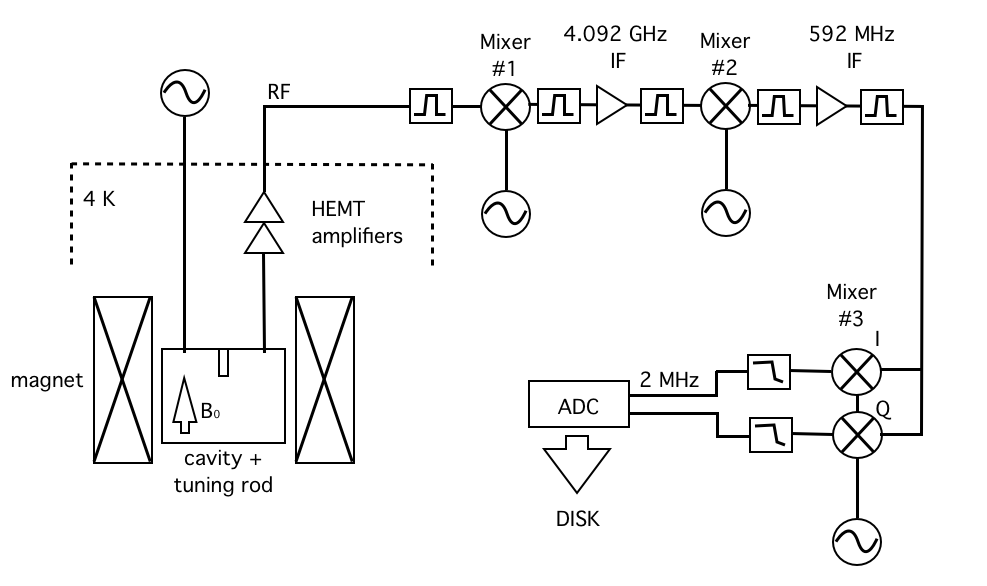
\includegraphics[width=\textwidth]{schematicnew}
\caption{Schematic of experiment}
\end{figure}

\begin{table}
\centering
\begin{tabular}{| c | c | c | c |}\hline
\hline
Component & Gain (dB) & \multicolumn{1}{|p{2cm}|}{\centering Power Density \\ (dBm/Hz)} & Total Power (dBm) \\ \hline \hline
Cavity & - & -185 & -  \\ \hline
Cryogenic Amplifiers w/ 3dB atten. & 50 & -144 & - \\ \hline
Waveguide to Shielded Room & -3.4 & -148.6 & -\\ \hline
RF switch & -2.7 & & \\ \hline
RF filter & -0.2 & - & -\\ \hline
RF mixer & -12 & x & x\\ \hline
Cable to Electronics & - & - & - \\ \hline
16 dB attenuation & -16 & - & - \\ \hline
1.5 GHz Bandpass Filter & -0.5 & - & - \\ \hline
4 GHz Amplifier & 59.5 & - & - \\ \hline
Bandpass Filter & -0.5 & - & - \\ \hline
4 GHz - 590 MHz Mixer & -6.5 & - & - \\ \hline
25 MHz Bandpass Filter & -2.3 & - & - \\ \hline
590 MHz Amplifier  & 34 & - & - \\ \hline
25 MHz Bandpass Filter & -2.3 & - & - \\ \hline
590 Mz to DC IQ Mixer & -8.5 & x & x \\ \hline
4 MHz Low Pass Filter & x & - & - \\ \hline
50 Ohm Voltage Pre-Amp  & x & - & - \\ \hline
\end{tabular}
\caption{Power levels at different points (in dBm) in the receiver chain. At each point in the receiver chain the total broadband noise power over the bandwidth of the next component is insufficient to cause saturation}
\label{table:rxchain}
\end{table}

\begin{table}[htdp]
\caption{Model Numbers}
\begin{center}
\begin{tabular}{|c|c|}
4GHz amp & MITEQ AFS33-04000420-20-10P-GW-44 \\ \hline
RF mixer & MITEQ M2640W1 \\ \hline
another amp & MITEQ AFS3-00100400-13-10P-4 \\ \hline
4GHz Filter & Spectrum Microwave 311-517144-001\\ \hline
4MHz filter & Spectrum Microwave 311-527062-001 \\ \hline
IQ mixer & MITEQ IR0502LC1Q
\end{tabular}
\end{center}
\label{default}
\end{table}%

A vacuum window is in place after the directional coupler which allows us to pump on the waveguide. Then comes a waveguide RF filter with a bandpass from 32.6-36 GHz. Then a waveguide to coax adaptor, and a a mechanical RF latching switch (RLC electronics 1 pole 2 throw). The custom receiver chain was designed by Penny Slocum, with three stages of mixing and bandpass filters to suppress image frequencies and harmonics. The image frequency is at $\omega_i = \omega_{LO} - \omega_{IF} = 2\omega_{LO}-\omega_{RF}$. The first LO comes from Anritsu MG3694C signal generator (so is tunable) with output power level of +15 dBm and goes to the mixer with conversion loss 12 dB that mixes the signal to the 4 GHz range. The image frequency for a 34.29 GHz RF signal would be 26 GHz (assuming LO mixes RF down to 4.09), which is attenuated by the waveguide RF filter. Then there are two cascaded amplifiers in the 4 GHz with total gain 60 dB (and a filter before and after them with width 1.5 GHz around a central frequency of 4.1 GHz), and second mixer with local oscillator fixed at 3.5 GHz. This mixes the signal down to around 590 MHz. Again, the image frequency is now 2.1 GHz. There is then another amplifier with 30 dB gain, and a 25 MHz filter around 590 MHz (again before and after the filter). The image frequency at this point is the same as the input frequency as we are mixing down to DC. The last mixer is an IQ mixer that mixes 590 MHz down to zero. There are two outputs, the I and Q channel, and each has a 4 MHz lowpass filter at the output. THe BNC outputs go to an SRS SR445A voltage pre-amplifier, set to 50 ohm input impedance and voltage gain of 5. This then goes to the PCI-5114 digitizer card, which samples at a 10 MHz rate set by the external digital clock with a resolution of 8 bits. The reference clock is the 10 MHz clock inside the signal generator which send out the first local oscillator signal.

\begin{figure}[htbp]
\includegraphics[width=\textwidth]{roomtempelectronicson}
\caption{Response of room temperature electronics chain}
\end{figure}

Once the signal is mixed down an offline script computes the discrete Fourier Transform to look at the voltage spectrum of the I and Q channels, the squared sum of which is the power spectral density. The Fourier Transform is computed using the FFTW libraries. For each spectrum, 294 samples were taken for each I, Q channel, yielding a 294 point power spectrum.

%The details of the mixing sequence are as follows: the first mixer has an LO input from a signal generator that can give out signals at frequencies up to 40 GHz. We usually set the LO to 30.2 GHz for RF signals to the input of 34.29 GHz. This would make the intermediate IF frequency around 4.09 GHz.There is then 60 dB of amplification and further filtering before the second mixer, which has a fixed LO frequency of 3.5 GHz. The IF then becomes 590 MHz. With more filtering and another 30 dB of amplification the 590 MHz signal enters an IQ mixer, which separates the in phase and quadrature components of the signal and mixes both down to baseband. There are two 25 MHz (or 4MHz) filters on the I and Q outputs, which determines the final bandwidth of our home made analyzer.
%
%All these elements are commercial and from MITEQ. The reason for filtering is to suppress image frequencies (frequencies $f_{image} = f_{LO}-f_{IF}$) since there are two frequencies that can mix down to the same intemediate frequency. The reason for the particular values of the local oscillator frequencies is that they are all multiples of 10 MHz so they can be all phase locked with a 10 MHz reference clock (in this case the clock is from the Anritsu signal generator) and the reason for the three stages of amplification is that these components seemed like a good idea.

The output power of the I channel after going through a voltage pre-amplifier is -97 dBm/Hz when looking at the thermal noise of a ~5 K cavity before the LNAs. The output power of the Q channel is usually -96 dBm/Hz. The difference between them are due to imperfections in the I/Q mixer.

\section{Data Acquisition and Analysis}
The data acquisition of the voltage time series controls the PCI digitizer card and sets the number of samples to acquire. This was written by Penny Slocum in C$\#$. 
%\begin{figure}[htbp]
%\includegraphics[width=\textwidth]{snapshotofdaq}
%\caption{The DAQ user interface. Written in C$\#$ by Penny Slocum, with minor adjustments made by me for logging and overflow problems. The DAQ digitizes the data and streams it to disk continuously, with $2.56\times10^6$ points per record acquired.}
%\end{figure}

Before running the data acquisition program, the cavity resonance is manually set and then the Q and bandwidth are measured with a vector network analyzer. Two microwave switches were installed to allow for the network analyzer to be directed to the cavity via the calibration waveguide, and also to allow test tone signals to be injected into the system.

The temperatures of various points along the cryostat are monitored continuously during data taking. One temperature sensor is connected to the bottom plate of the cavity, another to the first cryogenic amplifier, one connected to two points half way up the insert, and another on the vaporizer. The temperature sensors were produced and calibrated by Lakeshore Cryotronics Inc.  

%Five were used and they were attached at a) bottom plate of cavity, b)vaporizer c) cryogenic amplifiers, and d) two in the middle of the insert. The temperature sensors were calibrated to typically within a tenth of a degree Kelvin of the true temperature, and were read out with a temperature sensor controller also produced by Lakeshore.

%\begin{figure}[htbp]
%\includegraphics[width=\textwidth]{snapshotoftempmon}
%\caption{Written by Sergey Schkelunov. The Labview interface records the temperature of the sensors and plots the most recent points. A 50 ohm resistor is in place near the vaporizer. We use a power amplifier to and a heater control loop to control the temperature at the vaporizer. Practically speaking it is often more productive to wait until the cryostat has stabilized rather than try and use the heater to stabilize the temperatures.}
%\end{figure}




%\section{Data}
%
%To date we have performed two experiments - one using a single "quiet" cavity in the magnetic field, cooled to 4 K, and one using two cavities, with one quiet cooled cavity and the other driven by an RF source.

%The first experiment looked at the TE011 resonance (tunable but centered around 34.29 GHz) and tried to set a limit on the possible scalar particle-photon couplings that this setup could potentially detect. The starting assumptions are that the dark matter halo has a density of these scalar particles given by  $10^{13}$ GeV/${cm}^3$ which acts as the initial seed for these particle-photon conversions. The reason photon-particle conversions are not seen as a cancelling effect is that the number of photons is so much less than the number of particles that we have a huge population inversion $n_{ALP} >> n_{\gamma}$, and also that these conversions are so rare that a particle-photon-particle conversion and then reconversion would be suppressed by an extra factor of the weak coupling.
%
%The particle-photon conversion is stimulated by the presence of the strong magnetic field and enhanced in the region of a cavity, since there are fewer states that a cavity can support, therefore by Fermi's golden rule the transition probabilities of going from this continuum particle state to the discrete mode state of the photon are higher. This is known as the Purcell effect when talking about enhancement or suppression of spontaneous emission of an atom in a cavity.
%
%So the expression for the probability of conversion goes as the number of particles available to emit a photon (nV), the probability of a single particle conversion in free space with a magnetic field $(gB)^2$, the overlap integral expressing how likely the emitted photon is to be in the particular mode j we measure $(f_{j})$, and the enhancement by the Q of the cavity (Q). By conservation of angular momentum the emitted photon must have the same polarization as the magnetic field (really this is a two photon interaction, with the magnetic field providing a "virtual" photon), so since the magnetic field is axial, for a scalar interaction the emitted field must be a $TE$ mode (meaning the only axial field is magnetic, not electric).
%
%Therefore we have $P_{a\gamma} = (gB)^2 nfVQ.$ If the density is, as commonly the case, written as the energy density and not the number density we have $P_{a\gamma} = (gB)^2 n_e f_{j} VQ/m_a$, where natural units are assumed.
%
%Unfortunately the problem with looking for particles that give off photons whose wavepacket overlaps in a non-zero way with the $TE_{011}$ mode or in fact any $TE$ mode is that due to symmetry considerations, the overlap integral is in general very small or zero. The reason is because of boundary conditions -by Maxwell's equations the incident normal B field on a conductor must be zero, so for the axial magnetic field $B_z$, the boundary conditions imply $B_z(z=-L/2)=B_z(z=L) = 0$ so all $TE$ mode have an even $B_z$ field around $z=0$. But because of cylindrical symmetry, the value of $B_z(z,r=R)$ must be the same at diametrically opposed sides of the cylinder (at least for the lowest order mode). Because there are no magnetic monopoles, the magnetic field must integrate to zero. 
%
%As well, I was lying when I said $f_j$ goes as the integral of $B_z$. If you go through the equations of motion for Maxwell's equations with a source term of the form $B_z\cdot B_{magnet}$, the source term is actually second order with regards to $g$.
%
%Both of these things make it extremely hard to detect scalar particles in microwave cavities due to symmetry considerations and magnetic field properties.
%
%We nonetheless performed the experiment and were able to exclude $g > 10^{8}$ 1/GeV for masses $~0.14$ meV.

%The second experiment performed was for a two cavity detection method. Here the photon-particle-photon process is employed. By using an RF source as the photon source, we hope to produce these weakly interacting particles. Applying conventional shielding (any material) will attenuate the photons but not the particles. However to detect them we need to convert them back to regular photons. Since this process involves to extremely rare events, it suffers from the $g^4$ factor, but with a high intensity source of photons and using enhancement of the generation and detection volumes, one can improve the sensitivity to make experimentally interesting measurements. One caveat - having a high Q in the detection region will enhance sensitivity due to the Purcell effect as discussed above, but the Purcell effect is not what allows us to get enhancement by Q in the generation region. This is just due to the fact that the power in a cavity scales as the input power times Q.
%
%Instead of $f_j$ we now have $G$, the geometry factor, in the probability of this process occurring. $G$ takes into account the modes of each cavity and the distance between them.
%
%For vector particles, $G ~ 0.12$ for two $TE_{011}$ cavities separated by 3 cm. For scalar particles $G = $ I don't know for scalars, probably zero since the generation probability is zero. And of course zero for pseudoscalars which need a different polarization of the mode, since we were only looking at the $TE$ mode. However maybe it is non-zero for another mode.
%
%For this two cavity experiment, we drove one cavity $TE_{011}$ mode with a signal generator set for its maximum stable output of 22 dBm or 158 mW. The signal was a cw signal at the cavity resonance, usually 34.299 GHz, although it changed by about 300 KHz due to variations in room temperature. The bandwidth of the signal is very small, about 0.1 Hz. There was approximately a meter of waveguide between the cavity and the signal output, as well as a directional coupler and isolator between the two. At 34 GHz the loss of wr28 is 3 dB/m, and since the cavity was observed to be not critically coupled, there is probably more than 6 dB of power that does not get into the cavity. This changes the power entering the cavity to about 16 dBm, or around 30 mW. For a Q of  around 7,000,  this means that the power circulating in the cavity is in general around 210 Watts. Is this right? I am not sure, it seems to be wrong. Need to look at accelerator books and people who talk about RF power.
%
%As the cryostat is in the bore of the magnetic field, the driving cavity is also placed in the bore, next to the cryostat. Thus the walls of the driving cavity, the cryostat walls, and the walls of the quiet cavity all act as layers of attenuation for regular photons. We cool the quiet cavity down to 4 K to reduce the background thermal noise, and encase the electronics for mixing and analyzing the RF signal in a metal room which acts as a Faraday cage to close off any potential interference from the 22 dBm source.
%
%Our first measurements showed that there was an intermittent signal at our frequency of interest on the level of 3 dB above the thermal noise background. We had the driving cavity detuned with respect to the driving frequency $\omega_L$, so the observed spike, if from hidden photons would have to come from a process whith only one Q and a much lower G, since it would have to convert from the circular mode of the waveguide which connects to the cavity. So by suppressing any possible $\gamma'\rightarrow \gamma$ conversions, we test for interference exclusively. When the quiet cavity and driving cavity were retuned, the leak appeared to be larger, but still intermittent. We suspected that the interference was happening in the electronics, not through the cryostat or cavity. Two suspects were the power leads for the LNAs that could carry an RF signal down into the cryostat or the various connections in the mixing scheme which could pick up EM leakage. At room temperature with the LNAs powered off, the spike was observed but disappeared by closing the door to the shielded room encasing the electronics. At room temperature with the LNAs powered on ... this has not been tested.
%
%With the parameters in our setup we were able to place an exclusion limit on the coupling of vector particles to photons for $\chi > 10^{-7}$ 1/GeV.


%Maybe some ideas would be trying to use metamaterials or do mode-locking somehow. I don't think our amplifiers have the bandwidth to support more than two, maybe three modes mode-locked and I haven't seen anything that says that people have tried to mode-lock microwave cavities, but this woud emit radiation at higher peak intensties because they would all be emitted in one short burst. I thought this would improve our 
%signal to noise but maybe it wouldn't because we only care about fluctuations in the signal and these are not different are they? I don't know.
%Also a way to get around the high frequency, small volume problem seems to be to make it not be a problem - ie find ways to make high volumes resonate at high frequencies in low order modes. So we need an anti-dielectric, which will increase the frequency rather than lower it. Dielectric smaller than one only exist as things called metamaterials and I don't know their RF properties.
%Or maybe mode-locked detectors could help us because of the thing of pulsed things having better signal to noise than cw things. Not really sure.


%\section{Receiver Noise Figure}
%
%Because of the Friis formula the noise in the entire electronics analyzing chain is dominated by the noise of the first amplifier if it's gain is high enough.

%\section{HSP Introduction}
%
%We also did a HSP search using two $\text{TE}_{011}$ cavities. There was one $\text{TE}_{011}$ cavity that was not tunable and had a resonant frequency of 34.29 GHz. It had one aperture coupling on the bottom face where it went to 13 mm cylindrical waveguide and then to WR28. There was a meter and a half of this between an isolator and directional coupler and before all of that a signal generator capable of putting out 25 dBm but in practice we operated it at 22 dBm because it would output a warning that the power was unleveled at 25 dBm. 
%
%There the reflected power went through the directional coupler to a spectrum analyzer.
%
%The $\text{TE}_{011}$ cavity (signal cavity I’ll call it) was inside the bore of the magnet but outside the cryostat
%
%SHOW SCHEMATIC OF EXPERIMENT
%
%EMI Shielding
%
%There are many shielding improvements made iteratively. I list them below:
%
%1. Aluminum Wool in Bore of Magnet
%2. Copper Tape Over Joints of WR28 connections
%3. Copper tape over Vacuum Tube connections in Shielded Room
%4. Terminator on Cable to Weak Port when Disconnected
%5. HEMT power supplies moved to different room than both magnet and shielded room
%6. Everything locked to 10 MHz reference
%7. Shielded Room Shut and Run on Battery Power
%8. 10 MHz BNC cable hole drillled in shielded room wall and had RF absorbing foam placed around opening
%9. Aluminum Wool Placed in Holes leading HEMT power supply cables out.
%10. One HEMT power supply grounded through another HEMT power supply.
%
%\section{Expected Sensitivity}
%
%As the power is monochromatic, by reducing the resolution bandwidth we decrease the noise in each bin while the power stays the same. The size of each resolution bandwidth is inversely proportional the number of samples we acqure, and thus the integration time. The exact formula is 
%
%resBW = 1/tau
%
%When no windowing is used.
%
%\section{Thermal Noise - As Expected?}
%
%\section{Hypothesis Testing}
%
%\section{HSP Results}
%
%Hopefully we can redo these results, but we were able to make an exclusion based on non-observation of a peka in a 2.5 minute run.
%
%\begin{figure}
%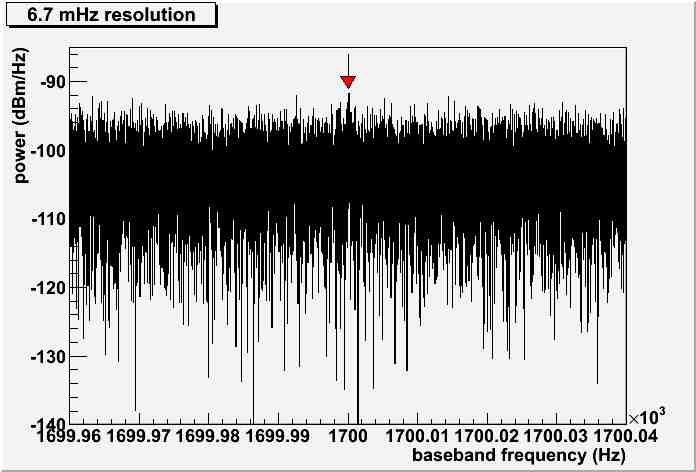
\includegraphics[scale=0.3]{malagon_ana_fig2}
%\end{figure}
%\begin{figure}
%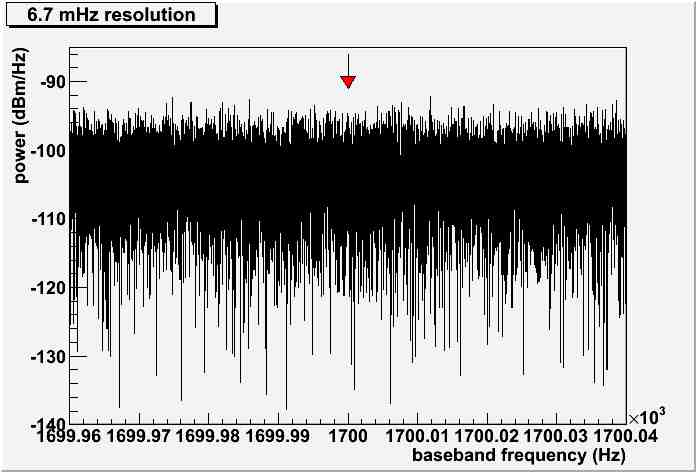
\includegraphics[scale=0.3]{malagon_ana_fig3}
%\end{figure}
%
%\begin{figure}
%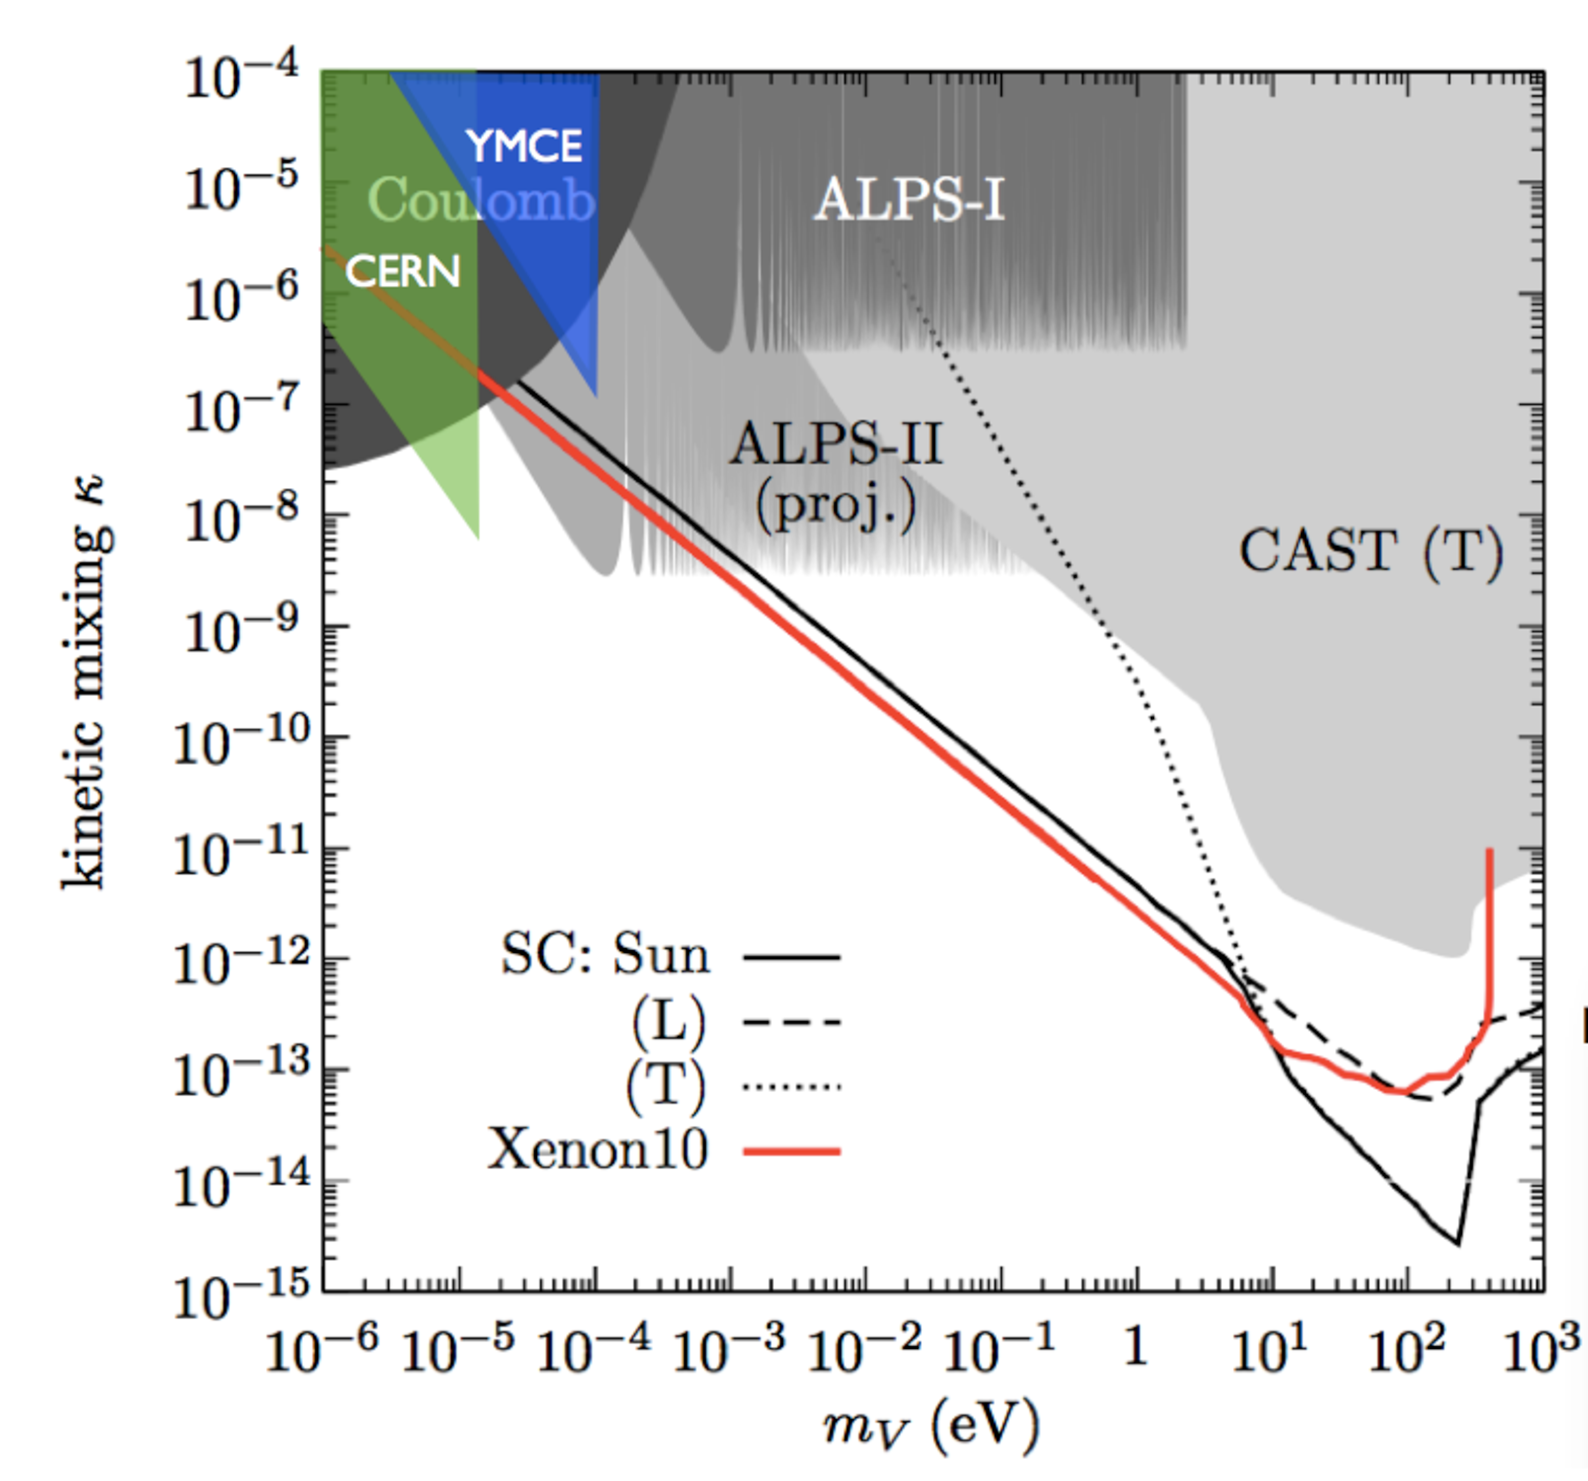
\includegraphics[scale=0.3]{malagon_ana_fig4}
%\end{figure}



%\section{Signal injection}
%
%It would be advantageous to inject a synthetic axion line int othe experiment cavity. the benefits are simple, we could test different search algorithms and determine their relative performance without the need for Monte Carlo methods in the data analysis. The scheme for inject this synthetic signal is simple and is sketched in Figure 3.
%
%The synthetic axion line would be injected into the cavity during data taking via the weakly coupled minor port. 

%I've demonstrated that a single synthetic axion line can be injected into the cavity and detected with the receiver chain. The next step would be to calibrate the power level of the injected signal inside the cavity from the noise power and then automate the procedure. With sufficient statistics the search confidence can be validated by search algorithms to be discussed in Chapter 4.


%\section{Data Runs}
\begin{figure}[htbp]
\includegraphics[width=\linewidth]{frequencycoveragepretty}
\caption{The first runs were taken with a slow DAQ that operated with 60$\%$ deadtime. The runs taken at 33.4 GHz had the cavity filled with helium. A heater feedback loop was put in place and an RF switch installed to toggle between the network analyzer and the receiver. In April 2014 the insert was taken out to study the dead spot between 33.368-33.398 GHz. Andrew Martin discovered it was due to the weak coupling port being so weakly coupled that at those frequencies no power was entering the cavity. The coupling was raised by adding a 20 thousandths metal shim in the bottom of the waveguide, adjusting the effective coupling.}
\end{figure}

%We used a cylindrical cavity cooled to $\sim 5$ K resonant at a frequency of $33.9-34.5$ GHz in the $\text{�}_{020}$ mode. The cavity was tuned to a specific resonant frequency using a dielectric rod; we measured the resonant frequency and Q using a vector network analyzer, then recorded the amplified noise from the cavity (after being mixed down to baseband) for an hour before retuning the cavity by 3 MHz. The baseband noise when Fourier transformed is a measure of the power in each frequency interval $\delta f$ that is the sum of the power in the cavity plus additional noise from the receiver chain. 

%We recorded data in twelve separate runs (Nov 19 to May 30, 2014), and measured noise for 500 settings of the cavity frequency, with an hour of integration. The actual performance of our system

%Summary of Runs
%\begin{center}
%\begin{tabular}{c | c | c }\hline
%\hline
%Run & No. of Freq.'s & State \\ \hline \hline
%11/19-11/22 & 9 & slow DAQ \\ \hline
%12/03-12/07 & 39 & faster DAQ \\ \hline
%12/10-12/13 & 22 & tuning rod froze\\ \hline
%12/16-12/20 & 27 & RF switch added\\ \hline
%01/08-01/11 & 46 & heater feedback loop online\\ \hline
%01/14-01/18 & 69 & 00 \\ \hline
%01/23 & 5 & -- \\ \hline
%01/28-02/01 & 41 & test tone added \\ \hline
%02/04-02/07 & 33 & tuning rod froze\\ \hline
%02/11-02/13 & 19 & -- \\ \hline
%03/10-03/13 & 16 & -- \\ \hline
%05/06-05/09 & x & weak coupling port altered, test tone removed\\ \hline
%05/14-05/17 & x & -- \\ \hline
%05/28-05/30 & x & -- \\ \hline
%\hline
%\end{tabular}
%\label{table:runsummary}
%\end{center}

\subsection{Procedure during normal running}

The data acquisition system (computer plus sensors plus instruments) measures important parameters, e.g. temperatures, pressures. As discussed earlier, the important cavity parameters are the cavity quality factor Q, center frequency of the cavity, strength of magnetic field, and cavity physical temperature. Once these quantities are measured, we manually tune the tuning rod by an amount corresponding to 3 MHz (approximately xx length). The cavity resonance moves, the cavity parameters are then measured, and then a 1 hr time trace is acquired as a two channel system and saved to disk in little-endian binary format as signed 8-bit integers.

%The binary data format compresses the information by a factor of xx in relation to ASCII (Text) format. The data format is as follows: there is a xx byte header, followed by the 2948-bit integers plus three FFT parameters. The following table shows the axion data format taken for these data.
%
%There is a potential issue in saving data with one computer and then post-processing the data on another. Data might be "big endian" or "little endian", referring to the byte order of how floating point numbers are read by different computer platforms. The mismatch was solved with a byte swapping routine, which first checked whether the data made sense if the data was in one endian form or another. Once established, the endian issue is resolved and the post-processing computer performs the analysis.

\begin{table}
\centering
\begin{tabular}{| c | c ||}\hline
\hline
Description & size (bytes) \\ \hline
Header & 35 \\ \hline
Gain & x \\ \hline
Offset & x \\ \hline
NumSamples &  xs\\ \hline
NumTriggers & x \\ \hline
Voltage(T) & x \\ \hline
\end{tabular}
\caption{Data format for YMCE running. Each file begins with four numbers specifying the digitizer gain, offset, number of triggers, and number of points in each trigger. It is followed by a header and then the 294 points for the time record}
\label{table:dataformat}
\end{table}

%\subsection{State Parameters}

%Below is a plot of the measured loaded Q over the runs taken.
\begin{figure}[htbp]
\centering
\includegraphics[width=1\textwidth]{loadedQ}
\caption{Q as measured by the VNA E8364C over the course of the runs. The runs with unusually low Q, near 5000, were taken near the "dead spot". After the shim was inserted in the cavity weak port waveguide, these runs were retaken and the Q was normal (near 8000).}
\end{figure}

%\section{Temperature Drifts}
%Another danger is if the cavity gets liquid in it, the resonance is no longer stable. This is probably because it fills up very slowly due to a small but intermittent leak somewhere in the indium seals of the waveguides. This means that whenever we saw the temperature sensors reading less than 4 K, we usually stopped the run and heated the cavity up. Thirdly, we found that the stability of the cavity resonance was more robust to changes if the cavity was at a higher temperature - changes of .5 K at 10 K seemed to affect the cavity resonance much less than at 5 K. One explanation is that the pressure in the cavity altered the resonance frequency - from John Rogers Thesis \cite{rogers87}, in their experiment they saw that there was a 30 kHz/GHz/psi shift. We see a XXX shift.


\section{Cool-down Troubleshooting}

During a typical cool down, we pumped out the sample region and pumped on the cryostat vacuum jacket for several days prior to the run. Then we filled the sample region and capillary tube with helium until the following test was satisfied: in opening the valve which allowed pumping on the sample region, the pressure rose to 10 Torr within 10 seconds. This generally meant that the region had only helium gas in the region. 

The nitrogen reservoir is then filled using the autofill system. This is set to refill every 3-4 hours. We then filled the helium reservoir, which has a capacity of 3 Liters. Depending on the state of the cryostat, the helium consumption can be .75 L/hr or .25 L/hr. We generally found that the lower helium consumption was tied to longer pumping times on the cryostat vacuum, however the temperature of the room and humidity also mattered. As well, we generally had more success with temperature stability after several rounds of helium fills.

It typically took three to four hours for the vaporizer (at the bottom of the cryostat) to reach liquid helium temperatures. At that point the liquid helium was usually depleted and another fill was done. After two fills, we are usually able to begin taking data, although the top of the cryostat continues to cool down, making temperature stability in the first day tricky. 

A heater feedback control loop was implemented in Labview, however, as the flow valve does not have a fine regulator, it is difficult to predict the helium flow rate in each cool down, so regular adjustment of the feedback loop was necessary.  The vaporizer was usually held between 3 and 4 Kelvin; when the vaporizer went below that it was usually a sign of liquid accumulating in the bottom. 

If the cavity temperature drops below 4 Kelvin, this is also a sign of liquid accumulating in the cavity. This can be due to a vacuum leak allowing helium gas to enter the cavity and waveguide assembly and then condensing. Although having liquid in the cavity on first thought seems like a good way to achieve temperature stability, in practice we tried to avoid this state, as the cavity frequency is no longer stable, but moves back and forth every few seconds by around 0.5 MHz. This oscillation may be due to helium boiling in the cavity; the combination of liquid accumulating and bubbles  due to boil-off disturbing the liquid make for an unstable state. 

The waveguide leading from the calibration port of the cavity to the shielded room has a directional coupler attached to it. We use a vacuum feedthrough attached to the coupling port of the directional coupler to pump on the waveguide during cool-downs. This can reduce the chance of liquid accumulation by decreasing the pressure of gas inside the cavity.

\section{Dead Spot}

Between 33.368 and 33.398 GHz the cavity resonance disappears. We initially believed this to be due to a mode crossing, even though no other modes are visible, and though it might be due to a mode that usually didn't couple to the waveguide being excited. However, the cause turned out to be the extremely weak coupling of the calibration port suppressing the mode at that frequency.

\begin{figure}[htbp]
\begin{subfigure}{\textwidth}
\includegraphics[width=\textwidth]{1stpic}
\caption{The cavity response is suppressed at the edge of this band and no response is apparent in the middle of the dead spot.}
\end{subfigure}
\begin{subfigure}{\textwidth}
\includegraphics[width=\textwidth]{2ndpic}
\caption{Resonance severly suppressed. Taken Feb 05, 2014.}
\end{subfigure}
\end{figure}

However after adding the metal shim in the bottom of the waveguide, the cavity resonance re-appears in this region.

\begin{figure}[htbp]
\begin{subfigure}{\textwidth}
\includegraphics[width=\textwidth]{1stpic_1_}
\end{subfigure}
\begin{subfigure}{\textwidth}
\includegraphics[width=\textwidth]{2ndpic_1_}
\end{subfigure}
\caption{May 07, 2014 - cavity response looks normal after inserting a shim and setting frequency to previously problematic region.}
\end{figure}

\section{Data Analysis}
\subsection{Introduction}
The previous chapter explained the setup of the experiment. We now discuss the analysis of the data, where we looked for peaks in the recorded spectra.  In the absence of statistically significant peaks, we set a limit on the minimum detectable power we can measure, and use that as our exclusion limit. 

%In our analysis, we assume that the axion has a boosted Maxwellian distribution with energy fractional width of $\mathcal{O}(10^{-6}$, or about one 34 KHz bin. 

The analysis process can be decomposed into three parts: baseline corrections, weighting and peak finding.

In section 4.2 we show the procedure for correcting the raw data and cuts made. Section 4.3 discusses the power combining and resulting exclusion limit, section 4.4 describes the resulting candidates and section 5 shows our final exclusion result.

\section{Data Processing}


In a typical run, we sampled voltage as a function of time from two channels in our receiver chain over the course of an hour. At a sampling rate of 10 MHz/sec, this generated a large volume (37 GB  per channel) of data. Using the FFTW libraries \cite{fftw} we computed the discrete Fourier transform for each set of 294 samples. Squaring the voltage transforms and summing resulted in a power spectra. The double-sided power spectra has a span of -5 to 5 MHz, centered at 0 MHz. Each spectra is saved to a file which consists of two vectors corresponding to the baseband frequency and power density, respectively. The first step in data analysis is to extract axion induced signals (i.e. peaks) from raw spectra. As we are searching for extremely weak signals amidst the noise, searching for true signals is a challenging task. 

An axion induced signal would appear as a local maxima in the spectra. However, detecting the signal is challenging as a the weakness of the signal means it may be buried by noise, causing a high false positive rate of peak detection. For each cavity setting, we average over many spectra to increase our sensitivity. As well, electronic noise results in a curve that affects the background of the data, which is referred to as a baseline. THe existence of the baseline produces strong  bias in the peak detection. It is desirable to remove the baseline before peak detection.

\begin{figure}[htbp]
\includegraphics[width=\linewidth]{flowchart2}
\caption{Data Analysis Pipeline}
\end{figure}

\section{Baseline correction}

Baseline correction is typically a two-step process: (1) estimating the baseline and (2) subtracting the baseline from the signal. In the following, we list details of the method we used to calculate the baselines using smoothing filters.

\subsection{Smoothing Filters}

For an input spectrum, we represent it as [f,p] with the first element as the frequency bin vector and the second element as the power spectral density (with equal length). We use p[n] to denote the discrete form of the power density vector. The input spectrum is always discrete. A spectrum after smoothing can be expressed as $y[n] = x[n] * w[n]$ where $*$ denotes the convolution operation. In the above equations, $w[n]$ is a weight vector. The use of different $w[n]$ will lead to different filters.

\subsection{Moving average filter}

The baseline was initially estimated using a moving average filter, where the output of the moving average filter $y[n]$ is defined as:

\begin{align*}
y[n] = x[n] * w[n] = \frac{1}{2k+1}\Sigma_{i=-k}^{k} x[n-i]
\end{align*}

where $w[n] = \frac{1}{2k+1}$, $-k \leq n \leq k$ a. The odd number $2k+1$ denotes filter width. The greater the filter width, the more intense the smoothing effect. However, this filter failed to remove oscillatory structure that appears at the level of $O(10^{-3})$. Shown below is the residual after using the moving average to calculate the baseline and then averaging over 522 baseline-removed traces.

This structure is much wider than our expected signal; therefore, we attempt to correct for it using a different filter, known as a Savitzky-Golay filter. The Savitsky-Golay filter can be considered as a generalized moving average filter. It performs a least squares fit of a small set of consecutive data points to a polynomial and takes the central point of the fitted polynomial curve as output.

The smoothed data point $y[n]$ after the Savitzky-Golay filtering is given by the following equation:

\begin{align*}
y[n[ = x[n] * w[n] = \frac{\Sigma A_i x[n-i]}{\Sigma A[i]}
\end{align*}

Using the Savitzky-Golay filter with a polynomial order of 4 and window size of 11 points reduces the residual structure significantly.

\begin{figure}[htbp]
\begin{subfigure}{\textwidth}
\includegraphics[width=0.8\linewidth]{01-11-08-24-55avgsubpltposfreq_522}
\caption{Systematic residual structure seen when baseline is estimated using moving average filter.}
\end{subfigure}
\begin{subfigure}{\textwidth}
\includegraphics[width=0.8\linewidth]{01-11-08-24-55gs-avgsubpltposfreq_522}
\caption{Residual when baseline is estimated using Savitzky-Golay filter.}
\end{subfigure}
\end{figure}

\section{Data Description}

We use data from measurements taken between 12/13 and 6/14. The physical temperature of the cavity was between 4 and 10 K. The observation time for each cavity setting was on average 1.06 hours. For data taken between Jan 29 2014 and March 13 2014, a test tone signal was injected into the cavity. The test tone frequency was set to be mixed down to -1 MHz. For these runs the cavity frequency was normally mixed down to 2 MHz. 

This data set has 499 groups of data. Each group has a number of spectra, usually 261. 
%\section{Running Time}
%
%\section{Parameter Tuning}
%
%\section{Conclusion}
%
%\begin{table}
%\centering
%\begin{tabular}{| c | c | c | c |}\hline
%\hline
%Component & Gain (dB) & \multicolumn{1}{|p{2cm}|}{\centering Power Density \\ (dBm/Hz)} & Total Power (dBm) \\ \hline \hline
%Cavity & - & -185 & -  \\ \hline
%Cryogenic Amplifiers w/ 3dB atten. & 50 & -144 & - \\ \hline
%Waveguide to Shielded Room & -3.4 & -148.6 & -\\ \hline
%RF switch & -2.7 & & \\ \hline
%RF filter & -0.2 & - & -\\ \hline
%RF mixer & -12 & x & x\\ \hline
%Cable to Electronics & - & - & - \\ \hline
%16 dB attenuation & -16 & - & - \\ \hline
%1.5 GHz Bandpass Filter & -0.5 & - & - \\ \hline
%4 GHz Amplifier & 59.5 & - & - \\ \hline
%Bandpass Filter & -0.5 & - & - \\ \hline
%4 GHz - 590 MHz Mixer & -6.5 & - & - \\ \hline
%25 MHz Bandpass Filter & -2.3 & - & - \\ \hline
%590 MHz Amplifier  & 34 & - & - \\ \hline
%25 MHz Bandpass Filter & -2.3 & - & - \\ \hline
%590 Mz to DC IQ Mixer & -8.5 & x & x \\ \hline
%4 MHz Low Pass Filter & x & - & - \\ \hline
%50 Ohm Voltage Pre-Amp  & x & - & - \\ \hline
%\end{tabular}
%\caption{Power levels at different points (in dBm) in the receiver chain. At each point in the receiver chain the total broadband noise power over the bandwidth of the next component is insufficient to cause saturation}
%\label{table:rxchain}
%\end{table}

The measurements from Dec 2013 to May 2014 were taken at 368 distinct resonant frequencies, with 499 total observations made. 415 of these observations were taken for 1.06 hours, with a smaller number (28) being taken for longer observation times; the remaining observations were taken for shorter times due to storage limitations or technical problems with the data acquisition system, and later were retaken to increase the number of averages at that frequency setting. For each measurement we tracked the in-phase and quadrature components of the baseband signal, and converted the time-domain data into a 294 bin,  34013.6 Hz/bin double-sided FFT power spectra. The FFT traces are 10 MHz wide, with a center frequency at 0Hz. Each of the spectra consist of 500,000 averages lasting a total of 14.7 seconds in integration time; for the standard observation length of 1.06 hrs, 261 such spectra could be produced. 

\begin{figure}[htbp]
\centering
\includegraphics[width=\textwidth]{examplespectra}
\label{fig:example}
\caption{FFT Power spectral density vs baseband frequency. Each bin is 34013.6 Hz wide.}
\end{figure}

Shown in Figure\ref{fig:example} is one such raw FFT trace. The horizontal axis shows the baseband frequency, and the vertical axis corresponds to the power density across the 50 ohm input in milliWatts per Hz. The visible features in the spectrum are the spike at 0 Hz, which is DC noise, the skirts at the edges showing the attenuation of the last low pass filter in the receiver chain, the 1/f noise near the center, and a dip corresponding to the combined cavity-amplifier response.

\subsection{Corrections}

To remove the features due to the last low-pass filter, we cut out the first and last thirty bins of each trace to remove the filter skirts, and also cut out twenty bins around the center to remove the DC spike and 1/f noise. 

%\begin{figure}[htbp]
%\centering
%\includegraphics[width=\textwidth]{roomtempchain1}
%\label{fig:roomtempchain1}
%\caption{The transfer function of the room temperature electronics chain with the RF switch in place, for different settings of the first local oscillator.}
%\end{figure}

The first local oscillator of the receiver is usually set so that the cavity resonant frequency is mixed down to 2 MHz. However, for a period of runs the first local oscillator was set so that the cavity frequency was mixed down to -1 MHz or -0.5 MHz in the baseband. There are also some measurements that had to be discarded because the local oscillator frequency was incorrectly set due to operator error and thus the cavity frequency was outside of the pass-band of the last filter. In order to prevent this from occurring, we introduced a test tone signal at an RF frequency such that it would mix down to -1 MHz, to make sure the local oscillator was set correctly. For the measurements taken with the test tone on, we later also cut out the bin with the test tone signal, as well as the two nearest bins to either side, for reasons to do with the fit. Lastly, there is some leakage into the positive frequency bins at 1 MHz due to the test tone; this will be discussed later.

\begin{figure}[htbp]
\begin{subfigure}{0.5\linewidth}
\includegraphics[width=\textwidth]{rawwithtesttone}
\caption{FFT trace with test tone signal at 34.044 GHz, -60 dBm}
\end{subfigure}
\begin{subfigure}{0.5\textwidth}
\includegraphics[width=\textwidth]{rawwithtesttone2}
\caption{FFT trace with test tone signal at 34.258 GHz, -72 dBm}
\end{subfigure}
\label{fig:testtone}
\end{figure}

\begin{figure}[htbp]
\centering
\includegraphics[width=0.85\textwidth]{rawwithfit2}
\label{fig:dataandfit}
\caption{FFT trace and fit.}
\end{figure}

We then estimate the baseline as described in the previous section and cut the seven bins at the end of the spectrum as well as the seven bins nearest the gap. This is to guard against end effects when computing the smooth. The baseline is subtracted from the data to give the residual fluctuations.

\begin{figure}[htbp]
%\centering
\begin{subfigure}[b]{0.5\textwidth}
\includegraphics[width=1.15\textwidth]{meansub}
\label{fig:ms}
\caption{Residual}
\end{subfigure}
\begin{subfigure}[b]{0.5\textwidth}
\includegraphics[width=\textwidth]{02-12-04-36-35gs-avgsubplt_75}
\label{fig:avgsubplt}
\caption{Average of 75 residual traces.}
\end{subfigure}
\hfill
\begin{subfigure}[b]{0.5\textwidth}
\includegraphics[width=1.1\textwidth]{meansubzoomed}
\label{fig:msz}
\caption{Residual trace in cavity region\ for one FFT trace}
\end{subfigure}
\begin{subfigure}[b]{0.5\textwidth}
\includegraphics[width=\textwidth]{02-12-04-36-35gs-avgsubpltposfreq_75}
\label{fig:avgsubpltpos}
\caption{Average of 75 residual traces, cavity region. Test tone leakage at 1 MHz.}
\end{subfigure}
\end{figure}
For frequency bins in the FFT trace that are outside of the 3 dB bandwidth of the cavity, the bins can be considered as holding purely background noise. Therefore, when the cavity is centered at 2 MHz in the baseband, this means that we drop all bins occurring at negative frequencies.

The shape of the data near the cavity resonance is dictated by the interaction of the cavity and amplifier coupling, as described in the previous chapter.

\begin{figure}[htbp]
\begin{minipage}{0.5\linewidth}
\includegraphics[scale=0.38]{12-12-15-39-55gs-withfitposfreq_261}
\vspace{4ex}
\end{minipage}
\begin{minipage}{0.5\linewidth}
\includegraphics[scale=0.38]{02-12-04-36-35gs-withfitposfreq_75}
\vspace{4ex}
\end{minipage}
\begin{minipage}{0.5\linewidth}
\includegraphics[scale=0.38]{01-11-12-06-17gs-withfitposfreq_261}
\vspace{4ex}
\end{minipage}
\begin{minipage}{0.5\linewidth}
\includegraphics[scale=0.38]{05-29-05-50-37gs-withfitposfreq_261}
\vspace{4ex}
\end{minipage}
\label{fig:varofcurve}
\caption{Data with fits for different resonant frequencies}
\end{figure}

Ref \cite{dawthesis98} describes the equivalent circuit model of the cavity and amplifier. The result is a five parameter model that can be used to fit the measured data. We are able to fit the data successfully using the five parameter model, but find practically that the empirical fit is more convenient to use. As well, the empirical fit removes the residual oscillatory structure which arises due to the room temperature electronics.

The $\delta P$ power fluctuations that result from the fit subtraction form the data that we analyze to look for excess power.

After subtracting the fit from each FFT trace, we average together many such corrected FFT traces. Within the standard observation time of 1.06 hrs, there were usually 261 FFT traces. Because temperature and pressure variations cause the cavity frequency to shift during the hour of data taking as discussed in the previous chapter, all the FFT traces produced were inspected, and if there was a significant shift in the structure of the traces over the hour, those significantly different traces were discarded. 

There is also leakage at the level of $0.5\%$ of the test tone power into the bins near 1 MHz. This is due to incomplete isolation in the IQ mixer, which is responsible for separating out the in-phase and quadrature components of the signal. The test tone was present in 105 measurements. We gradually reduced the power level of the test tone, but for 72 of the observations, the leakage was statistically significant and so we cut the out the five bins around 1 MHz as well.

\begin{figure}[htbp]
\includegraphics[width=\textwidth]{leakage15}
\caption{Shown are the output power for a test tone sent in at -60 dBm and the power leakage in the 1 MHz bin. For an hour of integration time, the power fluctuations are $O(10^{-14})$, so the test tone leakage is significant.}
\end{figure}


%\begin{figure}[h]
%\begin{subfigure}{0.5\linewidth}
%\includegraphics[width=1\textwidth]{02-04-14-03-57}
%\caption{Change in power spectra over course of 20 min run.}
%\end{subfigure}
%\begin{subfigure}{0.5\linewidth}
%\includegraphics[width=0.8\textwidth]{temp02-04-14-03-57}
%\caption{Temperature of system (red = 1st amplifier, blue = cavity) over run.}
%\end{subfigure}
%\label{fig:tempdrift}
%\caption{We discard data when temperature drifts or frequency drifts occur.}
%\end{figure}

By taking 65 bins considered to measure only background noise and looking at the distribution of fluctuations for 261 traces after correcting for the baseline, we see that the distribution is Gaussian. The width of the Gaussian is $2.45*10^{-13} \text{ mW}/\text{Hz}$ in terms of the output power spectral density; if we convert this to thermodynamic temperatures by dividing out the gain of the system (87 dB) and Boltzmann's constant, we see $\sigma =  .034$ K, which is consistent with the radiometer equation value of $\sigma = T_{sys}/\sqrt{N} = 20/\sqrt{5\times10^5} = 0.028$ K.

This gives us confidence that the statistics of the noise are indeed Gaussian. Thus we assign an initial uncertainty to each bin $i$ in the FFT trace of magnitude $\sigma = P_i/\sqrt{N}$, where $P_i$ is the power of the $i$th bin.

\begin{figure}[htbp]
\includegraphics[width=\linewidth]{01-16-11-30-28gs-histogramofleftbins_261}
\label{fig:singlegaussian}
\caption{Histogram of power fluctuations from 261 corrected FFT traces (baseline), taking the fluctuations from 65 background bins from each trace.}
\end{figure}

As we average the corrected FFT traces together, the fluctuations should go down as $t^{-1/2}$, or as the square root of the number of averages $1/\sqrt{N}$. To estimate this, we take the bins which do not survive the final cut of ``region of interest``; that is to say, for a cavity centered at 2 MHz, we take the residual baseline portion for the negative frequency bins, and by calculating the standard error of the mean as a function of the number of averaged FFT traces that go into the residual baseline, we can get an estimate of whether the system is behaving according to Gaussian statistics. The reason we take the negative (or opposite) frequency bins is to make sure we are only looking at background noise.

\begin{figure}[htbp]
\includegraphics[width=\linewidth]{gs-logstderr1}
\label{fig:stderr}
\caption{The standard error of the mean of the background bins (92 bins) vs number of averages for a stable 5 hour run}
\end{figure}
% for the timestamp 05-30-23 
%The residual baseline for many runs shows a systematic error, showing that we have not fully removed all structure. The amplitude of this effect appears at the level of $0.1\%$.

Figure \ref{fig:std err} shows that the log of the standard error does indeed go down linearly as we increase the number of averages. This was done for a five hour run; we can see that for that integration time, we have not yet hit a systematic noise floor.

%The total number of averages in each frequency bin is between 0.2 and 2 $10^9$.

\section{Lorentzian Correction}

After correcting the FFT traces for the baseline, we apply an additional weight to the power fluctuations and uncertainty of each bin to remove the cavity response. This factor corrects for the fact that an axion produced off resonance will have a signal amplitude attenuated by the Lorentzian response of the cavity. By weighting by the inverse response, the signal height is expected to be the same in each bin, barring differences in different runs due to different quality factors and form factors. We apply this weighting to the uncertainty of each bin as well.

\begin{align*}
h(f) = \frac{1}{1+4(f-f_0)^2/\Gamma^2}
\end{align*}

\begin{figure}[htbp]
\centering
\begin{subfigure}{0.78\textwidth}
\includegraphics[width=\linewidth]{05-16-12-15-04gs-avgsubplt_92}
\caption{FFT trace with cuts in place and baseline removed. 92 traces are averaged together.}
\end{subfigure}
\begin{subfigure}{0.78\textwidth}
\includegraphics[width=\linewidth]{05-16-12-15-04gs-avgsubpltlc_92}
\caption{FFT trace with cuts in place and baseline removed and cavity response divided out. 92 traces are averaged in this plot.}
\end{subfigure}
\label{fig:lorentz}
\end{figure}

Figure \ref{fig:lorentz} shows the effect of dividing out the cavity Lorentzian. 
\section{Combining Power Spectra}

For power spectra with overlapping frequency bins, we average the power values at those bins from the different traces, with weights given by the inverse uncertainty squared. This weighting gives the maximum likelihood for the mean of values with non-uniform uncertainties. For more discussion on this topic, see \cite{daw89}, \cite{yu04}. The physical intuition behind doing the weighted arithmetic mean is that it allows us to favor bins which have smaller uncertainties because the temperature was lower in that run or because more traces were averaged together at that setting.

\[
\bar{ \delta P_f} = \Sigma_r \delta P_{r, f} w_{r,f}
\]
\[w_{r,f} = \Sigma_r 1/\sigma_{r,f}^2/A\]
\[A=\Sigma_r w_{r,f}\]

So the combined power fluctuations $\bar{ \delta P_f}$ are the weighted mean of the power fluctuations from runs $r$ at the frequency f: $\delta P_{r,f}$, each of which has uncertainty $\sigma_{r,f}$. $A$ is the overall normalization. 

An RF switch was added between the waveguide and receiver chain at the end of Dec 20, 2013. This introduced a loss of 2.55 $+ .67$ $-.79$ dB over the frequency range scanned. Therefore we correct for the difference in gain by dividing all runs taken before the switch was introduced by a factor of 1.8.

The histogram of the power fluctuations in the co-added power spectrum is compared with a simulation done by adding Gaussian noise to the baseline curves and otherwise running it through the data analysis pipeline in the same manner as the real data. Both the real data and simulation have a Gaussian distribution; however the distribution of the real data is narrowed with respect to the simulation distribution. This may be due to the effect of the baseline removal.

\begin{figure}[htbp]
\centering
\includegraphics[width=0.9\linewidth]{histogramofcoaddedpowerspectrum2}
\caption{Histogram of power fluctuations in the total co-added power spectrum.}
\end{figure}

\begin{figure}[htbp]
\includegraphics[width=\linewidth]{numberofaverages}
\label{fig:numberofaverages}
\caption{The number of individual spectra that contribute to each frequency bin in the co-added power spectrum.}
\end{figure}

%\begin{figure}[htbp]
%\includegraphics[width=\linewidth]{lorentzcorrectednumberofaverages}
%\caption{Lorentz corrected number of traces contributing to each frequency}
%\end{figure}

\section{Threshold}

Although the noise is not perfectly Gaussian, we use Gaussian statistics to define a simple threshold. To test for outliers, we set the threshold at each bin $i$ equal to $3\sigma_i$ and rescan at all points where the bin value exceeds this threshold. 

\begin{figure}[htbp]
\includegraphics[width=\linewidth]{switchcorrected5-threshold-error}
\caption{Setting the threshold to be 3 times the uncertainty of each bin, there are 30 candidates.}
\end{figure}

The number of rescans $n_r$ we expect for Gaussian noise when setting a threshold of p sigma and looking at N bins is 
\[n_r = \frac{N}{2}(1-\text{erf}(\frac{p}{\sqrt{2}}))\]
 which for 18345 bins gives $n_r = 25$.

As oulitiers due to noise should go down with increasing averages, we covered the candidate frequencies with half an hour runs and produced a new co-added power spectrum with the rescans added into the data analysis pipeline. If the new co-added power value at the frequency is less than the original threshold, we consider the candidate to have been due to noise.

As all outliers were later suppressed due to additional data taken by rescanning the frequencies in the table above, we generate an exclusion limit by taking the minimum detectable axion signal power as the threshold value at each frequency and converting that into an axion-photon coupling.

%The fraction of power from the axion signal power that appears in a bin is a function of the distance between the axion frequency f_a and the center of the bin $f$ where the bin width is $\delta f$ : \Delta = 2(f_a - f)/\delta f$. For $\Delta > 0$, some fraction of the power leaks into adjacent bins due to the discrete nature of the transform; when $\Delta =1$ the signal is at the bin edge. This fraction of power is given by $P_a(\Delta) - \frac{4P_a}{\pi^2\Delta^2} \sin^2(\frac{\pi \Delta}{2})$. The probability of a signal passing the $3\sigma$ threshold for an offset $\Delta$ is
%
%\begin{align*}
%\begin{multline}
%Prob(P_a(\Delta) > 3) =\frac{1}{2\pi} \int_{-\infty}^{P_a(\Delta) - 3} exp(\frac{-x^2}{2}),\ dx
%= \frac{1}{2} (\frac{1+\text{erf}(P_a(\Delta) - 3}{\sqrt{2})
%\end{multline}
%\end{align*}
%
%Averaging over $\Delta \in [0,1]$
%
%
%\begin{align*}
%\overline Prob(P_a > 3 = \frac{1}{2} \int_{\Delta=0}^{\Delta=1} d\Delta (1+\text{erft}(\frac{1}{\sqrt{2}(P_a sinc^2(\pi \Delta/2) - 3)))
%\end{align*}

\begin{figure}[htbp]
\includegraphics[width=\linewidth]{numberofcandidatesvsthreshold2}
\caption{Number of candidates versus threshold}
\end{figure}

\begin{table}[htbp]
\caption{Candidates}
\begin{center}
\begin{tabular}{|c|c|c|}
\hline 
Frequency (GHz) & PSD (mW/Hz) & Threshold \\ \hline
33.922278828 & 2.6433062220 & 3e-14 2.56177873618e-14\\ \hline
33.9821087504 & 4.01889850759e-14 &  3.75779859252e-14\\ \hline
34.032823028 & 3.9813823045e-14 & 3.22466144484e-14\\ \hline
34.0330951368 & 3.57069525293e-14 & 3.19619691831e-14\\ \hline
34.0335713272 & 2.44207326219e-14 & 1.94152529304e-14\\ \hline
34.0352720072 & 1.88003796249e-14 & 1.82006596004e-14\\ \hline
34.0439794888 & 4.02448855563e-14 & 2.21003268442e-14\\ \hline
34.0585713232 & 2.25485631512e-14 & 2.04846595321e-14\\ \hline
34.0614284656 & 3.28436642257e-14 & 2.84855312922e-14\\ \hline
34.0632652 & 3.16572898809e-14 & 2.2479112676e-14\\ \hline
34.0662583968 & 2.87516371617e-14 & 2.33616496463e-14\\ \hline
34.1129930832 & 1.59198873493e-14 & 1.3809913528e-14\\ \hline
34.1426189288 & 4.16770641435e-14 & 3.78242771001e-14\\ \hline
34.1448298128 & 2.30593607493e-14 & 1.91897857856e-14\\ \hline
34.1449318536 & 2.03901772311e-14 & 1.85352212317e-14\\ \hline
34.1458502208 & 1.92768292095e-14 & 1.62473638403e-14\\ \hline
34.1463944384 & 1.70908654746e-14 & 1.69355141309e-14\\ \hline
34.1475168872 & 2.22833996376e-14 & 2.1356105071e-14\\ \hline
34.1725508968 & 2.90983734422e-14 & 2.24914699629e-14\\ \hline
34.1742515768 & 7.20190044285e-14 & 2.09515421745e-14\\ \hline
34.2082651768 & 3.08782413537e-14 & 2.68277290415e-14\\ \hline
34.2452719736 & 2.28537708519e-14 & 1.82106093843e-14\\ \hline
34.2590814952 & 2.38090356895e-14 & 2.05178958959e-14\\ \hline
34.3315644768 & 1.33971266806e-14 & 9.12957448161e-15\\ \hline
34.3332651568 & 8.30755776663e-15 & 5.97072478179e-15\\ \hline
34.338265156 & 1.99348483186e-14 & 1.88348838013e-14\\ \hline
34.3485712768 & 2.06439988028e-14 & 1.91898996061e-14\\ \hline
34.3699998448 & 2.39983850695e-14 & 2.32990970718e-14\\ \hline
34.5108501624 & 3.96664566965e-14 & 3.1224174159e-14\\ \hline
34.5175508416 & 1.57719161032e-14 & 1.56830081055e-14\\ \hline
34.5192515216 & 1.30334171873e-14 & 1.24182640031e-14\\ \hline
\end{tabular}
\end{center}
\label{default}
\end{table}%

An alternative approach is to estimate the noise by taking the local standard error of 1000 bins in the combined power spectrum, and then set the threshold as 3 times that local standard error. This approach has a lower threshold and thus more candidates arise. 

There are 78 bins with values greater than this threshold. 

\begin{figure}[htbp]
\includegraphics[width=\linewidth]{switchcorrected5-threshold-dots}
\caption{Number of candidates appearing when threshold defined using running standard deviation with window size of 1000.}
\end{figure}

There were two environmental signals that persisted after rescans.

SHOWENVIRONMENTALSIGNALS

In both, the corresponding negative frequency bin also showed an excess.

\section{Exclusion Limit}

From the threshold, we can derive an exclusion limit with $95\%$ confidence. For the first approach using the uncertainty in each bin to set the threshold, we can translate the output power into an expected axion-photon coupling. Our data analysis procedure is excluding axion signals that appear as power excesses in one bin. However, we must correct for the fact that if the axion converts to a photon whose frequency is not centered on the FFT bin, due to the discrete nature of the transform, some power is lost to other bins. In the worst case $40.5\%$ of the power is lost when the axion signal is at the boundary between two bins. We assume that this worst case scenario always happens by putting this factor in to the expected signal power, which degrades the exclusion result by $\sqrt{.405}$ or $16\%$. 

Assuming all the candidates end up being shown to be noise, we can set an exclusion limit as shown in the following figure.

\begin{figure}[htbp]
\includegraphics[width=\linewidth]{exclusionlimit-errorthreshold}
\end{figure}

This improves on the previous best limit in this frequency range by the CAST experiment of $g_{a\gamma\gamma} > 8.8 \times 10^{-11}$.

The confidence level can be obtained by finding the probability of a an axion signal passing the $3\sigma$ cut for a given offset from the center of a bin, and integrating over the various possible offsets.

SHOWCONFIDENCELEVELDIAGRAM

For a $90\%$ confidence level in total, we need the signal to pass both cuts with $\sqrt{.9} = .949$ probability, so the power level corresponding to a $95\%$ probability is some number of sigma.

A two bin search is slightly more sensitive, since in the worst case only $81\%$ of the power remains in any given two-bin. Again, we can take the worst case estimate as the valuation for all bins and set a limit 

SHOW2BINLIMIT

%\section{Procedure during normal running}
%
%The data acquisition system (computer plus sensors plus instruments) measures important parameters, e.g. temperatures, pressures. As discussed earlier, the important cavity parameters are the cavity quality factor Q, center frequency of the cavity, strength of magnetic field, and cavity physical temperature. Once these quantities are measured, we manually tune the tuning rod by an amount corresponding to 3 MHz (approximately xx length). The cavity resonance moves, the cavity parameters are then measured, and then a 1 hr time trace is acquired as a two channel system and saved to disk in little-endiant binary format as signed 8-bit integers.
%
%The binary data format compresses the information by a factor of xx in relation to ASCII (Text) format. The data format is as follows: there is a xx byte header, followed by the 2948-bit integers plus three FFT parameters. The following table shows the axion data format taken for these data.
%
%There is a potential issue in saving data with one computer and then post-processing the data on another. Data might be "big endian" or "little endian", referring to the byte order of how floating point numbers are read by different computer platforms. The mismatch was solved with a byte swapping routine, which first checked whether the data made sense if the data was in one endian form or another. Once established, the endian issue is resolved and the post-processing computer performs the analysis.
%
%\begin{table}
%\centering
%\begin{tabular}{| c | c ||}\hline
%\hline
%Description & size (bytes) \\ \hline
%Header & 35 \\ \hline
%Gain & x \\ \hline
%Offset & x \\ \hline
%NumSamples &  xs\\ \hline
%NumTriggers & x \\ \hline
%Voltage(T) & x \\ \hline
%\end{tabular}
%\caption{Data format for YMCE running. Each file begins with four numbers specifying the digitizer gain, offset, number of triggers, and number of points in each trigger. It is followed by a header and then the 294 points for the time record}
%\label{table:dataformat}
%\end{table}
%\section{Sensors and Instrumentation}
%
%The experiment relied on a number of important sensors, mostly temperature sensors, level sensors, and vacuum pressure sensors. One temperature sensor as connected to the bottom plate of the cavity, another to the first cryogenic amplifier, one connected to two points half way up the insert, and another on the vaporizer. The temperature sensors were produced and calibrated by Lakeshore Cryotronics Inc.  Five were used and they were attached at a) bottom plate of cavity, b)vaporizer c) cryogenic amplifiers, and d) two in the middle of the insert. The temperature sensors were calibrated to typically within a tenth of a degree Kelvin of the true temperature, and were read out with a temperature sensor controller also produced by Lakeshore.
%
%Vapor pressure of Helium 4. 
%
%\section{The FFT}
%
%The FFTW libraries are used to do the data reduction. Uniform windowing is employed. Figure 4 shows a typical averaged power spectrum taken during running.
%
%The most obvious feature of this typical power spectrum is the rapid falloff in power outside the frequency range -4-4 MHz, caused by attenuation outside the passband of the low-pass 4 MHz filter. Understanding the shapes of traces from the raw data is important for data analysis since the signal from axions is predicted to be power excess over a bin of a trace above the noise baseline. Treatment of the noise baseline is presented in chapter 4.
%
%\section{Signal injection}
%
%It would be advantageous to inject a synthetic axion line int othe experiment cavity. the benefits are simple, we could test different search algorithms and determine their relative performance without the need for Monte Carlo methods in the data analysis. The scheme for inject this synthetic signal is simple and is sketched in Figure 3.
%
%The synthetic axion line would be injected into the cavity during data taking via the weakly coupled minor port. 
%
%I've demonstrated that a single synthetic axion line can be injected into the cavity and detected with the receiver chain. The next step would be to calibrate the power level of the injected signal inside the cavity from the noise power and then automate the procedure. With sufficient statistics the search confidence can be validated by search algorithms to be discussed in Chapter 4.
%
%\section{Input match of the first cryogenic amplifier}
%
%To measure the input match of the 1st cryogenic amplifier, the power reflection coefficient at room temperature was determined according to the apparatus of Figure 3.
%
%The signal from the sweeper is incident on the load via the directional bridge. Power reflected off the load is directed onto a power sensor. A null measurement is first done with the bridge terminated in a short so all the incident RF power is reflected. Next the short is replaced with the device under test. The difference between the reflected power with the amplifier connected and the reflected power with the short connected is the the power reflection coefficient.  Figure 3 is the power reflection coefficient as a function of frequency. There vertical axis is the reflection coefficient in dB with the cursor indicating 0 dB and 4 dB per division.
%
%The power reflection coefficient is very good, better than -18 dB over a bandwidth of at least 799 MHz. The reflection coefficient is not expected to have a strong temperature dependence and any serious worsening of the reflection coefficient would manifest itself through poor gain and high noise temperature. As we shall see from the results of cryogenic measurements later in this section, at low temperatures the gain of the amplifier increases and its noise decreases, indicating that the good match at the amplifier input persists at cryogenic temperatures.
%
%\section{The first cryogenic amplifier coupled to the resonant cavity}
%
%If the load on the cavity is not a 50 ohm impedance then a fraction of this power reflects off the load and appears back at the amplifier as a signal. Since the cavity impedance is rapidly varying with frequency near resonances it is important to understand the contribution of the internal terminations to the system noise with a cavity  connected to the amplifier input.
%
%The following experiment is an indicator of how noise sources in the amplifier contribute to the amplifier noise with a cavity load. The cryogenic amplifier is critically coupled to the resonant cavity at room temperature. The power spectrum a the amplifier output is measured using a spectrum analyzer, first with the amplifier at room temperature then with the amplifier cooled in liquid nitrogen. Figure 3 shows the two power spectra.
%
%Consider the upper trace, taken when the cavity was warmer than the amplifier. On resonance the cavity acts as a load perfectly matched to the amplifier input. Therefore all power from the amplifier that is emitted at the input port is absorbed in the cavity and not reflected. The noise temperature at the input is the physical temperature of the cavity.
%
%\section{The gain of the cryogenic amplifiers at cryogenic temperatures}
%
%It is important to make an 'in situ' measurement of the gain of the first cryogenic amplifier and the results compared with gain data supplied by Sandy Weinreb. The gain of the cryogenic amplifier was measured previously uon a cold test-stand.
%
%\subsection{'In Situ' measurement of the cryogenic amplifier noise temperature}
%
%The noise temperature of the 1st cryogenic amplifier was measured with the amplifier installed on the axion receiver. We argued in the previous section that the 1st cryogenic amplifier is the only component in the receiver chain whose noise temperature significantly affects the sensitivity of the search. This measurement is a check that the amplifier noise temperature in the high magnetic field of the detector remains low.
%
%The amplifier noise temperature is referenced to the temperature of the Johnson noise in the cavity. The cavity temperature is varied, and by looking at the output power of the cryogenic amplifier as a function of the cavity temperature, the amplifier noise temperature can be deduced.
%
%Referring to figure 3, the cryogenic amplifier is critically coupled to the cavity using the reflection method described earlier. For the remainder of the measurement, the directional coupler is not used. On-resonance, the impedance of the cavity through the critically coupled probe is 50 ohms. Hence the cavity may be used as a source of thermal noise at a known temperature. The cavity temperature is initially 1.6 K.
%
%The cavity is warmed by allowing the pressure above the liquid helium lake below the cavity to rise. A large gate valve between the Roots blower and the insert space is closed most of the way to allow for a slower pressure relaxation. As the helium vapor pressure rises, the temperature of the liquid helium also rises, until at atmosphere pressure, the physical temperature of the liquid and the vapor helium inside the cavity space is 4.2 K. Care is taken to ensure the cavity warmup is slow. During this slow warmup the data acquisition runs.
%
%The DAQ software first injects a swept signal through the weak port and measures the transmission to the receiver chain using a network analyzer, then takes a power spectrum about the cavity resonance. Figure 3 shows the power per Hz for the on-resonance bin versus temperature for our in situ noise temperature measurement for a cavity resonant frequency of xx GHz. Specifically, the output power at the end of the axion receiver is given by 
%
%Noise temperature versus frequency from Sander Weinreb.
%
%\begin{figure}[htbp]
%\includegraphics[width=0.5\textwidth]{yfactor5}
%\caption{Y-factor measurement of the 1st HEMT noise done using a 50 Ohm load in a copper block. We heated the block quickly and used a short stainless steel segment in order to thermally isolate the hot block from the HEMT. The plot shows  the  output power measured over a resolution bandwidth of 3 MHz on the spectrum analyzer as a function of frequency.}
%\end{figure}
%
%\begin{figure}[htbp]
%\includegraphics[width=0.5\textwidth]{yfactor6}
%\caption{Noise Temperature}
%\end{figure}
%
%\begin{figure}[htbp]
%\includegraphics[width=0.5\textwidth]{weinrebgain}
%\caption{Gain of 1st amplifier measured by vendor}
%\end{figure}
%
%Let us neglect the effect of the waveguide to coaxial adaptor. Then the noise at the input of the 1st cryogenic amplifier is the sum of the load and amplifier physical temperatures plus the intrinsic electronic noise temperature of the amplifier:
%
%$T_{sys} = T_{HEMT} + T_{load} + T_N$
%
%If we assume that the noise temperature of the amplifier remains constant over a small range of physical temperatures, say 4-10 K, then by doing the Y-factor measurement with the HEMT at approximately the same temperature and the load temperature varied, we see that 
%
%$T_{sys,hot load} - T_{sys, cold load} = \Delta T_{HEMT} + \Delta T_{load}$ 
%
%Unfortunattely it is difficult to make noise temperature measurements of the cryogenic amplifier in situ to an accuracy of better than 10 percent. This is due to difficulty in controlling the exact temperature of the resonant cavity as it warms. However, our value measured in situ is consistent with the value measured by Sander Weinreb. We used 10 K as our amplifier noise temperature for the frequency range 33.9-34.5 GHz.
%
%\section{The room temperature electronics}s
%
%After the signal leaves the first cryogenic amplifier, it goes through a 3 dB attenuator and a second cryogenic amplifier. After this it proceeds up the waveguides in the insert through a feedthrough, through more waveguides, past a vacuum window and through a waveguide to coax adaptor and to the room temperature electronics. We discuss the room temperature electronics in this section.
%
%\subsection{RF components}
%
%The output of the 
%=====
%BELOW THIS POINT IS OLD WORK
%
%We used a cylindrical cavity cooled to $\sim 5$ K resonant at a frequency of $33.9-34.5$ GHz in the $\text{�}_{020}$ mode. The cavity was tuned to a specific resonant frequency using a dielectric rod; we measured the resonant frequency and Q using a vector network analyzer, then recorded the amplified noise from the cavity (after being mixed down to baseband) for an hour before retuning the cavity by 3 MHz. The baseband noise when Fourier transformed is a measure of the power in each frequency interval $\delta f$ that is the sum of the power in the cavity plus additional noise from the receiver chain. 
%
%We recorded data in twelve separate runs (Nov 19 to May 30, 2014), and measured noise for 500 settings of the cavity frequency, with an hour of integration. The actual performance of our system
%
%Summary of Runs
%\begin{center}
%\begin{tabular}{c | c | c }\hline
%\hline
%Run & No. of Freq.'s & State \\ \hline \hline
%11/19-11/22 & 9 & slow DAQ \\ \hline
%12/03-12/07 & 39 & faster DAQ \\ \hline
%12/10-12/13 & 22 & tuning rod froze\\ \hline
%12/16-12/20 & 27 & --\\ \hline
%01/08-01/11 & 46 & heater feedback loop online\\ \hline
%01/14-01/18 & 69 & RF switch added \\ \hline
%01/23 & 5 & -- \\ \hline
%01/28-02/01 & 41 & test tone added \\ \hline
%02/04-02/07 & 33 & tuning rod froze\\ \hline
%02/11-02/13 & 19 & -- \\ \hline
%03/10-03/13 & 16 & -- \\ \hline
%05/06-05/09 & x & weak coupling port altered, test tone removed\\ \hline
%05/14-05/17 & x & -- \\ \hline
%05/28-05/30 & x & -- \\ \hline
%\hline
%\end{tabular}
%\label{table:runsummary}
%\end{center}
%\section{Procedure}
%the following section is formed of quotes/notes from Silk(?) in "Inner Space Outer Space"
%We tracked the in-phase and quadrature voltage of our baseband signal for an hour at each frequency setting. To allow for overlap between the covered frequencies, the cavity resonance was shifted by 3 MHz at a time. The dominant systematic effects were temperature variations in the cryostat. 
%
%To reduce the effects of the the temperature shifts we discarded all data that was greater than 28 sigma away from the first minute of data. 
%
%The data presented here were taken during 2014 Nov 19-22, Dec 05 to 07, 11 to 13, � . These runs gave a total of 500 hours of useful data. After correcting the data for the gain of the receiver and converting them to thermodynamic temperatures we compute the mean values $\Delta T_{bin}^i$ for the observations of each frequency bin of width $\delta f$ for each spectrum. The corresponding standard deviations, $\sigma_{bin}^i$ are calculated from the scatter of the individual 57 second measurements and are an estimate of the statistical uncertainty in the mean of an hour of data. ADDINBOOTSTRAP A typical value for data taken at 5 K is $\sigma_{bin189}^i = 0.25 mK$ whereas one expects $0.14$ mK from system noise alone. The excess noise at this stage is due to the $1/f$ component and in the variable temperature noise.
%
%The final values $\bar \Delta T_{bin}^i$ for each one of the bins were obtained by weighting by $(\sigma_{bin}^i)^2$ each one of the hour observations for a given bin. The results are plotted in Figure 1 and show no statistically significant signal in any of the bins. The errors associated to each point correspond to the standard deviations estimated from the measurement statistics in the usual way. As the data will be used to decide what level of axion coupling is excluded by these measurements it is crucial to estimate the errors in Figure 1 accurately. The scatter in the values of $\Delta T_f^i$ for the different measurements could be larger than expected from the systematic effects. In principle, one could perform standard Chi-square tests for each one of the bins. Any such test would compare the scatter of the different observations of a given field with respect to the final value, with the corresponding values of $\sigma$. Let me emphasize that such a test does not depend on whether there is a true signal coming from the sky, as the scatter is computed with respect tone "local mean"; it is truly an instrumental Chi-square test. Figure 2 shows a histogram of the weighted residuals $(\Delta T - \bar \Delta T)\sigma$ for the observations. The histogram is reasonably gaussian with the a width that is consistent with what we would expect if all the scatter the values of $\Delta T$ with respect to their corresponding average value were due to fluctuations contained in $\sigma_i$. Indeed, the corresponding value of Chi-Square is of 78 with 75 degrees of freedom. Therefore, we conclude that it is legitimate to estimate the standard deviations $\bar \sigma$ in the standard way, as $\bar \sigma = [\Sigma \sigma^{-2}]^{-1/2}$. The variation of $\sigma$ frm bin to bin is mainly due to the different number of runs over which each frequency is observed. The weighted mean of the points in Figure 1 is $T_{avg} = 26 \pm 3 mk$.
%
%It follows from visual examination of Figure 1 that none of the points differs significantly from the mean. The question is then what limits do the data place on $g_a$ from the fact that we only see the scatter shown in Figure 1. The Neyman-Pearson lemma prescribes the optimal statistical estimator for testing the hypothesis that $g_a \neq 0$. The optimal statistic turns out to be essentially a weighted Chi-square test, which can be used to find out which values of $g$ are ruled out at a certain confidence level.
%
%\section{State Parameters}
%
%Below is a plot of the measured loaded Q over the runs taken. NEED TO UPDATE
%\begin{figure}[htbp]
%\centering
%\includegraphics[width=1\textwidth]{measuredqvsfrequencyinsitucutoutoutlierswithtitle}
%\end{figure}
%
%Below is a plot of the form factor, calculated by simulating the electromagnetic fields in the cavity using the HFSS software.
%\begin{figure}[htbp]
%\centering
%\includegraphics[width=1\textwidth]{formfactorvsfrequency}
%\end{figure}
%
%Shown below is a cross-sectional plot of the electric field in the z-direction for a dielectric rod with $\epsilon = 9.2$ inserted 0.028 inches into the cavity.
%
%\begin{figure}[htbp]
%\centering
%\includegraphics[width=0.8\textwidth]{efieldhfsssim28thou}
%\end{figure}
%
%Shown below is the frequency coverage NEED TO UPDATE
%
%\begin{figure}[htbp]
%\centering
%\includegraphics[scale=0.7]{frequencycoverage}
%\end{figure}
%
%\section{Data Analysis in Detail}
%The data analysis starts from the raw time traces. The receiver chain at the final step separates the signal into an in-phase and quadrature component using an IQ mixer. These two separated signals each go through a low pass filter with approximately 4 MHz bandpass, and then are amplified by a voltage pre-amplifier with a gain of 5. The output channels (labeled henceforth as I and Q) are then plugged into a PCI 1154 card on a Dell desktop and digitized at a rate of 10 MSa/sec, with a a digital external referene at 10 MHz. We have a data acquisition program written in Visual C$\#$ that acquires however many records we desire, with each record containing 2.56e6 samples. The data acquisition has zero deadtime. The regular running procedure is to take 15,000 records at one particular cavity setting, and then retune - 15,000 records takes 1.06 hrs. 
%Shown below is an example spectra
%
%\subsection{cuts}
%
%We discard all chunks that have the cavity drifting in frequency.
%
%\begin{figure}[htbp]
%\includegraphics[width=\textwidth]{01-16-00-38-43}
%\includegraphics[width=\textwidth]{temp01-16-00-38-43}
%\end{figure}
%\begin{figure}
%\includegraphics[width=\textwidth]{01-14-16-14-53}
%\includegraphics[width=\textwidth]{temp01-14-16-14-53}
%\end{figure}
%
%We also cut data when the temperature difference causes changes in the spectra.
%
%\begin{figure}[htbp]
%\includegraphics[width=\textwidth]{02-04-14-03-57}
%\includegraphics[width=\textwidth]{temp02-04-14-03-57}
%\end{figure}
%\begin{figure}
%\includegraphics[width=\textwidth]{02-04-17-34-58}
%\includegraphics[width=\textwidth]{temp02-04-17-34-58}
%\end{figure}
%
%
%
%\section{HFSS Design}
%
%\includegraphics[width=\textwidth]{tableofchoice}
%
%\includegraphics[width=0.6\textwidth]{tm020efield}
%
%\includegraphics[width=0.6\textwidth]{tm020magneticfield}
%
%\includegraphics[width=\textwidth]{waveguidefields}

\bibliographystyle{plain}
\bibliography{thesisbib}

\end{document}